%%%%%%%%%%%%%%%%%%%%%%%%%%%%%%%%%%%%%%%%%%%%%%%%%%%%%%%%%%%%%%%
%
% Welcome to Overleaf --- just edit your LaTeX on the left,
% and we'll compile it for you on the right. If you open the
% 'Share' menu, you can invite other users to edit at the same
% time. See www.overleaf.com/learn for more info. Enjoy!
%
%%%%%%%%%%%%%%%%%%%%%%%%%%%%%%%%%%%%%%%%%%%%%%%%%%%%%%%%%%%%%%%
\documentclass{article}
% Turn off page numbers
\pagestyle{empty}
\usepackage{atbegshi}% http://ctan.org/pkg/atbegshi
\AtBeginDocument{\AtBeginShipoutNext{\AtBeginShipoutDiscard}}
\usepackage{geometry}
\geometry{
 papersize={360mm, 360mm},
 total={170mm,257mm},
 left=5mm,
 top=5mm,
 }
\usepackage{tikz}
\begin{document}
\begin{center}

\tikzset{every picture/.style={line width=0.75pt}} %set default line width to 0.75pt        

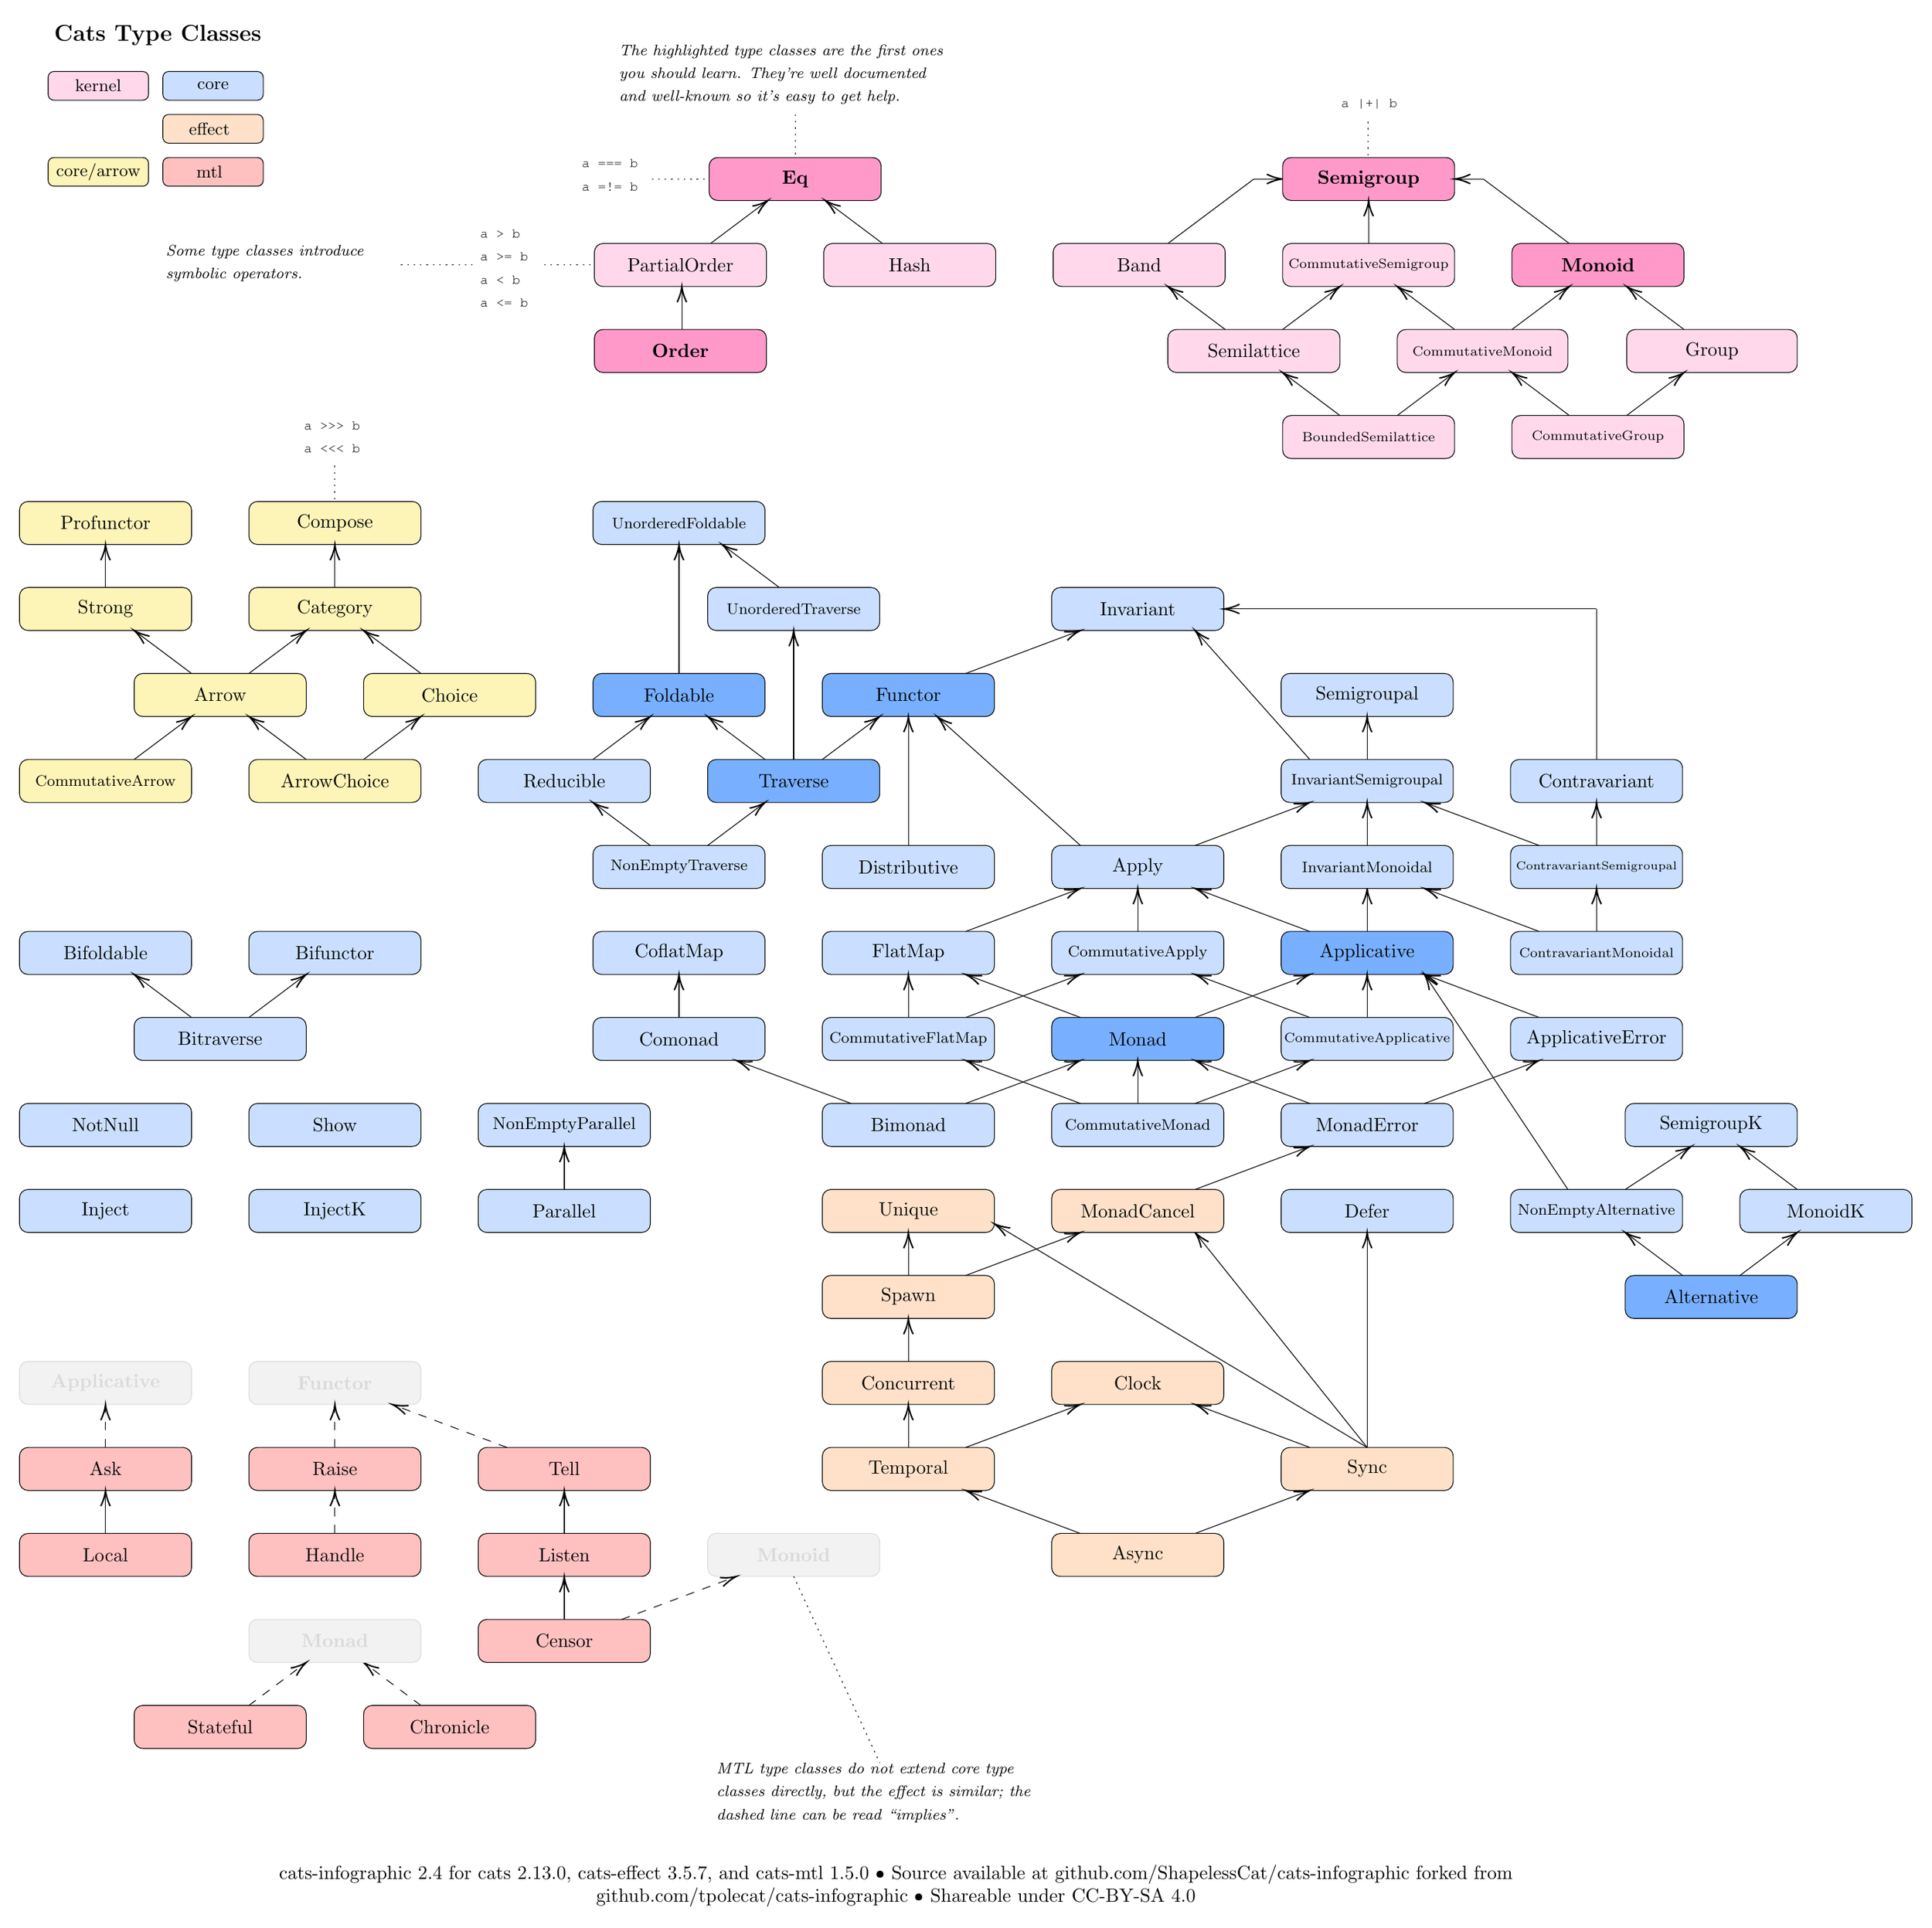
\begin{tikzpicture}[x=0.75pt,y=0.75pt,yscale=-1,xscale=1]
%uncomment if require: \path (0,1341); %set diagram left start at 0, and has height of 1341

%Rounded Rect [id:dp14911282011678795] 
\draw  [fill={rgb, 255:red, 255; green, 153; blue, 202 }  ,fill opacity=1 ] (491,116) .. controls (491,112.69) and (493.69,110) .. (497,110) -- (605,110) .. controls (608.31,110) and (611,112.69) .. (611,116) -- (611,134) .. controls (611,137.31) and (608.31,140) .. (605,140) -- (497,140) .. controls (493.69,140) and (491,137.31) .. (491,134) -- cycle ;

%Rounded Rect [id:dp8257795410681199] 
\draw  [fill={rgb, 255:red, 255; green, 217; blue, 235 }  ,fill opacity=1 ] (411,176) .. controls (411,172.69) and (413.69,170) .. (417,170) -- (525,170) .. controls (528.31,170) and (531,172.69) .. (531,176) -- (531,194) .. controls (531,197.31) and (528.31,200) .. (525,200) -- (417,200) .. controls (413.69,200) and (411,197.31) .. (411,194) -- cycle ;

%Rounded Rect [id:dp36916638243832645] 
\draw  [fill={rgb, 255:red, 255; green, 217; blue, 235 }  ,fill opacity=1 ] (571,176) .. controls (571,172.69) and (573.69,170) .. (577,170) -- (685,170) .. controls (688.31,170) and (691,172.69) .. (691,176) -- (691,194) .. controls (691,197.31) and (688.31,200) .. (685,200) -- (577,200) .. controls (573.69,200) and (571,197.31) .. (571,194) -- cycle ;

%Straight Lines [id:da7451515848291663] 
\draw    (492,170) -- (530.4,141.2) ;
\draw [shift={(532,140)}, rotate = 143.13] [color={rgb, 255:red, 0; green, 0; blue, 0 }  ][line width=0.75]    (10.93,-3.29) .. controls (6.95,-1.4) and (3.31,-0.3) .. (0,0) .. controls (3.31,0.3) and (6.95,1.4) .. (10.93,3.29)   ;
%Straight Lines [id:da3039114391772877] 
\draw    (612,170) -- (573.6,141.2) ;
\draw [shift={(572,140)}, rotate = 36.87] [color={rgb, 255:red, 0; green, 0; blue, 0 }  ][line width=0.75]    (10.93,-3.29) .. controls (6.95,-1.4) and (3.31,-0.3) .. (0,0) .. controls (3.31,0.3) and (6.95,1.4) .. (10.93,3.29)   ;
%Straight Lines [id:da33926113221748766] 
\draw    (472,230) -- (472,202) ;
\draw [shift={(472,200)}, rotate = 90] [color={rgb, 255:red, 0; green, 0; blue, 0 }  ][line width=0.75]    (10.93,-3.29) .. controls (6.95,-1.4) and (3.31,-0.3) .. (0,0) .. controls (3.31,0.3) and (6.95,1.4) .. (10.93,3.29)   ;
%Rounded Rect [id:dp1652319133624507] 
\draw  [fill={rgb, 255:red, 255; green, 153; blue, 202 }  ,fill opacity=1 ] (411,236) .. controls (411,232.69) and (413.69,230) .. (417,230) -- (525,230) .. controls (528.31,230) and (531,232.69) .. (531,236) -- (531,254) .. controls (531,257.31) and (528.31,260) .. (525,260) -- (417,260) .. controls (413.69,260) and (411,257.31) .. (411,254) -- cycle ;

%Straight Lines [id:da3108293800261901] 
\draw  [dash pattern={on 0.84pt off 2.51pt}]  (551,80) -- (551,110) ;
%Straight Lines [id:da696543957292195] 
\draw  [dash pattern={on 0.84pt off 2.51pt}]  (451,125) -- (491,125) ;
%Straight Lines [id:da4880747204592666] 
\draw  [dash pattern={on 0.84pt off 2.51pt}]  (376,185) -- (411,185) ;
%Straight Lines [id:da5224063746259779] 
\draw  [dash pattern={on 0.84pt off 2.51pt}]  (276,185) -- (326,185) ;

%Straight Lines [id:da2838816267112072] 
\draw    (871,125) -- (811,170) ;
%Straight Lines [id:da7657649291887403] 
\draw    (871,125) -- (889,125) ;
\draw [shift={(891,125)}, rotate = 180] [color={rgb, 255:red, 0; green, 0; blue, 0 }  ][line width=0.75]    (10.93,-3.29) .. controls (6.95,-1.4) and (3.31,-0.3) .. (0,0) .. controls (3.31,0.3) and (6.95,1.4) .. (10.93,3.29)   ;
%Rounded Rect [id:dp4165239073874165] 
\draw  [fill={rgb, 255:red, 255; green, 153; blue, 202 }  ,fill opacity=1 ] (891,116) .. controls (891,112.69) and (893.69,110) .. (897,110) -- (1005,110) .. controls (1008.31,110) and (1011,112.69) .. (1011,116) -- (1011,134) .. controls (1011,137.31) and (1008.31,140) .. (1005,140) -- (897,140) .. controls (893.69,140) and (891,137.31) .. (891,134) -- cycle ;

%Rounded Rect [id:dp08364601804858385] 
\draw  [fill={rgb, 255:red, 255; green, 217; blue, 235 }  ,fill opacity=1 ] (731,176) .. controls (731,172.69) and (733.69,170) .. (737,170) -- (845,170) .. controls (848.31,170) and (851,172.69) .. (851,176) -- (851,194) .. controls (851,197.31) and (848.31,200) .. (845,200) -- (737,200) .. controls (733.69,200) and (731,197.31) .. (731,194) -- cycle ;

%Rounded Rect [id:dp9361123405602181] 
\draw  [fill={rgb, 255:red, 255; green, 217; blue, 235 }  ,fill opacity=1 ] (891,176) .. controls (891,172.69) and (893.69,170) .. (897,170) -- (1005,170) .. controls (1008.31,170) and (1011,172.69) .. (1011,176) -- (1011,194) .. controls (1011,197.31) and (1008.31,200) .. (1005,200) -- (897,200) .. controls (893.69,200) and (891,197.31) .. (891,194) -- cycle ;

%Straight Lines [id:da5310299796079745] 
\draw    (1031,125) -- (1013,125) ;
\draw [shift={(1011,125)}, rotate = 360] [color={rgb, 255:red, 0; green, 0; blue, 0 }  ][line width=0.75]    (10.93,-3.29) .. controls (6.95,-1.4) and (3.31,-0.3) .. (0,0) .. controls (3.31,0.3) and (6.95,1.4) .. (10.93,3.29)   ;
%Rounded Rect [id:dp6719503907986937] 
\draw  [fill={rgb, 255:red, 255; green, 153; blue, 202 }  ,fill opacity=1 ] (1051,176) .. controls (1051,172.69) and (1053.69,170) .. (1057,170) -- (1165,170) .. controls (1168.31,170) and (1171,172.69) .. (1171,176) -- (1171,194) .. controls (1171,197.31) and (1168.31,200) .. (1165,200) -- (1057,200) .. controls (1053.69,200) and (1051,197.31) .. (1051,194) -- cycle ;

%Straight Lines [id:da6889998320646724] 
\draw    (1031,125) -- (1091,170) ;
%Straight Lines [id:da39023475570601374] 
\draw    (951,170) -- (951,142) ;
\draw [shift={(951,140)}, rotate = 90] [color={rgb, 255:red, 0; green, 0; blue, 0 }  ][line width=0.75]    (10.93,-3.29) .. controls (6.95,-1.4) and (3.31,-0.3) .. (0,0) .. controls (3.31,0.3) and (6.95,1.4) .. (10.93,3.29)   ;
%Rounded Rect [id:dp4151262537001972] 
\draw  [fill={rgb, 255:red, 255; green, 217; blue, 235 }  ,fill opacity=1 ] (811,236) .. controls (811,232.69) and (813.69,230) .. (817,230) -- (925,230) .. controls (928.31,230) and (931,232.69) .. (931,236) -- (931,254) .. controls (931,257.31) and (928.31,260) .. (925,260) -- (817,260) .. controls (813.69,260) and (811,257.31) .. (811,254) -- cycle ;

%Rounded Rect [id:dp23162322874561458] 
\draw  [fill={rgb, 255:red, 255; green, 217; blue, 235 }  ,fill opacity=1 ] (971,236) .. controls (971,232.69) and (973.69,230) .. (977,230) -- (1084,230) .. controls (1087.31,230) and (1090,232.69) .. (1090,236) -- (1090,254) .. controls (1090,257.31) and (1087.31,260) .. (1084,260) -- (977,260) .. controls (973.69,260) and (971,257.31) .. (971,254) -- cycle ;

%Rounded Rect [id:dp595037841698681] 
\draw  [fill={rgb, 255:red, 255; green, 217; blue, 235 }  ,fill opacity=1 ] (1131,236) .. controls (1131,232.69) and (1133.69,230) .. (1137,230) -- (1244,230) .. controls (1247.31,230) and (1250,232.69) .. (1250,236) -- (1250,254) .. controls (1250,257.31) and (1247.31,260) .. (1244,260) -- (1137,260) .. controls (1133.69,260) and (1131,257.31) .. (1131,254) -- cycle ;

%Straight Lines [id:da33509058137737036] 
\draw    (851,230) -- (812.6,201.2) ;
\draw [shift={(811,200)}, rotate = 36.87] [color={rgb, 255:red, 0; green, 0; blue, 0 }  ][line width=0.75]    (10.93,-3.29) .. controls (6.95,-1.4) and (3.31,-0.3) .. (0,0) .. controls (3.31,0.3) and (6.95,1.4) .. (10.93,3.29)   ;
%Straight Lines [id:da3031018272932433] 
\draw    (1011,230) -- (972.6,201.2) ;
\draw [shift={(971,200)}, rotate = 36.87] [color={rgb, 255:red, 0; green, 0; blue, 0 }  ][line width=0.75]    (10.93,-3.29) .. controls (6.95,-1.4) and (3.31,-0.3) .. (0,0) .. controls (3.31,0.3) and (6.95,1.4) .. (10.93,3.29)   ;
%Straight Lines [id:da9064905570697028] 
\draw    (1171,230) -- (1132.6,201.2) ;
\draw [shift={(1131,200)}, rotate = 36.87] [color={rgb, 255:red, 0; green, 0; blue, 0 }  ][line width=0.75]    (10.93,-3.29) .. controls (6.95,-1.4) and (3.31,-0.3) .. (0,0) .. controls (3.31,0.3) and (6.95,1.4) .. (10.93,3.29)   ;
%Straight Lines [id:da5817814103650507] 
\draw    (891,230) -- (929.4,201.2) ;
\draw [shift={(931,200)}, rotate = 143.13] [color={rgb, 255:red, 0; green, 0; blue, 0 }  ][line width=0.75]    (10.93,-3.29) .. controls (6.95,-1.4) and (3.31,-0.3) .. (0,0) .. controls (3.31,0.3) and (6.95,1.4) .. (10.93,3.29)   ;
%Straight Lines [id:da6486109322486326] 
\draw    (1051,230) -- (1089.4,201.2) ;
\draw [shift={(1091,200)}, rotate = 143.13] [color={rgb, 255:red, 0; green, 0; blue, 0 }  ][line width=0.75]    (10.93,-3.29) .. controls (6.95,-1.4) and (3.31,-0.3) .. (0,0) .. controls (3.31,0.3) and (6.95,1.4) .. (10.93,3.29)   ;
%Rounded Rect [id:dp5774516380894537] 
\draw  [fill={rgb, 255:red, 255; green, 217; blue, 235 }  ,fill opacity=1 ] (891,296) .. controls (891,292.69) and (893.69,290) .. (897,290) -- (1005,290) .. controls (1008.31,290) and (1011,292.69) .. (1011,296) -- (1011,314) .. controls (1011,317.31) and (1008.31,320) .. (1005,320) -- (897,320) .. controls (893.69,320) and (891,317.31) .. (891,314) -- cycle ;

%Straight Lines [id:da9226891540387663] 
\draw    (931,290) -- (892.6,261.2) ;
\draw [shift={(891,260)}, rotate = 36.87] [color={rgb, 255:red, 0; green, 0; blue, 0 }  ][line width=0.75]    (10.93,-3.29) .. controls (6.95,-1.4) and (3.31,-0.3) .. (0,0) .. controls (3.31,0.3) and (6.95,1.4) .. (10.93,3.29)   ;
%Straight Lines [id:da3551522952548978] 
\draw    (971,290) -- (1009.4,261.2) ;
\draw [shift={(1011,260)}, rotate = 143.13] [color={rgb, 255:red, 0; green, 0; blue, 0 }  ][line width=0.75]    (10.93,-3.29) .. controls (6.95,-1.4) and (3.31,-0.3) .. (0,0) .. controls (3.31,0.3) and (6.95,1.4) .. (10.93,3.29)   ;
%Straight Lines [id:da87960342688156] 
\draw    (1091,290) -- (1052.6,261.2) ;
\draw [shift={(1051,260)}, rotate = 36.87] [color={rgb, 255:red, 0; green, 0; blue, 0 }  ][line width=0.75]    (10.93,-3.29) .. controls (6.95,-1.4) and (3.31,-0.3) .. (0,0) .. controls (3.31,0.3) and (6.95,1.4) .. (10.93,3.29)   ;
%Straight Lines [id:da361290681981959] 
\draw    (1131,290) -- (1169.4,261.2) ;
\draw [shift={(1171,260)}, rotate = 143.13] [color={rgb, 255:red, 0; green, 0; blue, 0 }  ][line width=0.75]    (10.93,-3.29) .. controls (6.95,-1.4) and (3.31,-0.3) .. (0,0) .. controls (3.31,0.3) and (6.95,1.4) .. (10.93,3.29)   ;
%Straight Lines [id:da19326335758126412] 
\draw  [dash pattern={on 0.84pt off 2.51pt}]  (950.5,85) -- (950.5,110) ;
%Rounded Rect [id:dp3683172233037171] 
\draw  [fill={rgb, 255:red, 255; green, 217; blue, 235 }  ,fill opacity=1 ] (1051,296) .. controls (1051,292.69) and (1053.69,290) .. (1057,290) -- (1165,290) .. controls (1168.31,290) and (1171,292.69) .. (1171,296) -- (1171,314) .. controls (1171,317.31) and (1168.31,320) .. (1165,320) -- (1057,320) .. controls (1053.69,320) and (1051,317.31) .. (1051,314) -- cycle ;



%Rounded Rect [id:dp6524574125380747] 
\draw  [fill={rgb, 255:red, 202; green, 223; blue, 255 }  ,fill opacity=1 ] (410,596) .. controls (410,592.69) and (412.69,590) .. (416,590) -- (524,590) .. controls (527.31,590) and (530,592.69) .. (530,596) -- (530,614) .. controls (530,617.31) and (527.31,620) .. (524,620) -- (416,620) .. controls (412.69,620) and (410,617.31) .. (410,614) -- cycle ;

%Rounded Rect [id:dp10203714860032731] 
\draw  [fill={rgb, 255:red, 202; green, 223; blue, 255 }  ,fill opacity=1 ] (570,596) .. controls (570,592.69) and (572.69,590) .. (576,590) -- (684,590) .. controls (687.31,590) and (690,592.69) .. (690,596) -- (690,614) .. controls (690,617.31) and (687.31,620) .. (684,620) -- (576,620) .. controls (572.69,620) and (570,617.31) .. (570,614) -- cycle ;

%Rounded Rect [id:dp9340726473881562] 
\draw  [fill={rgb, 255:red, 202; green, 223; blue, 255 }  ,fill opacity=1 ] (410,656) .. controls (410,652.69) and (412.69,650) .. (416,650) -- (524,650) .. controls (527.31,650) and (530,652.69) .. (530,656) -- (530,674) .. controls (530,677.31) and (527.31,680) .. (524,680) -- (416,680) .. controls (412.69,680) and (410,677.31) .. (410,674) -- cycle ;

%Rounded Rect [id:dp17057166852232863] 
\draw  [fill={rgb, 255:red, 202; green, 223; blue, 255 }  ,fill opacity=1 ] (570,656) .. controls (570,652.69) and (572.69,650) .. (576,650) -- (684,650) .. controls (687.31,650) and (690,652.69) .. (690,656) -- (690,674) .. controls (690,677.31) and (687.31,680) .. (684,680) -- (576,680) .. controls (572.69,680) and (570,677.31) .. (570,674) -- cycle ;

%Rounded Rect [id:dp5401503874256464] 
\draw  [fill={rgb, 255:red, 202; green, 223; blue, 255 }  ,fill opacity=1 ] (410,716) .. controls (410,712.69) and (412.69,710) .. (416,710) -- (524,710) .. controls (527.31,710) and (530,712.69) .. (530,716) -- (530,734) .. controls (530,737.31) and (527.31,740) .. (524,740) -- (416,740) .. controls (412.69,740) and (410,737.31) .. (410,734) -- cycle ;

%Rounded Rect [id:dp18417818377909412] 
\draw  [fill={rgb, 255:red, 202; green, 223; blue, 255 }  ,fill opacity=1 ] (570,716) .. controls (570,712.69) and (572.69,710) .. (576,710) -- (684,710) .. controls (687.31,710) and (690,712.69) .. (690,716) -- (690,734) .. controls (690,737.31) and (687.31,740) .. (684,740) -- (576,740) .. controls (572.69,740) and (570,737.31) .. (570,734) -- cycle ;

%Straight Lines [id:da4480789289268443] 
\draw    (470,710) -- (470,682) ;
\draw [shift={(470,680)}, rotate = 90] [color={rgb, 255:red, 0; green, 0; blue, 0 }  ][line width=0.75]    (10.93,-3.29) .. controls (6.95,-1.4) and (3.31,-0.3) .. (0,0) .. controls (3.31,0.3) and (6.95,1.4) .. (10.93,3.29)   ;
%Straight Lines [id:da9230595438515843] 
\draw    (630,710) -- (630,682) ;
\draw [shift={(630,680)}, rotate = 90] [color={rgb, 255:red, 0; green, 0; blue, 0 }  ][line width=0.75]    (10.93,-3.29) .. controls (6.95,-1.4) and (3.31,-0.3) .. (0,0) .. controls (3.31,0.3) and (6.95,1.4) .. (10.93,3.29)   ;
%Rounded Rect [id:dp6733341242587592] 
\draw  [fill={rgb, 255:red, 202; green, 223; blue, 255 }  ,fill opacity=1 ] (730,596) .. controls (730,592.69) and (732.69,590) .. (736,590) -- (844,590) .. controls (847.31,590) and (850,592.69) .. (850,596) -- (850,614) .. controls (850,617.31) and (847.31,620) .. (844,620) -- (736,620) .. controls (732.69,620) and (730,617.31) .. (730,614) -- cycle ;

%Rounded Rect [id:dp19337240535501876] 
\draw  [fill={rgb, 255:red, 202; green, 223; blue, 255 }  ,fill opacity=1 ] (730,656) .. controls (730,652.69) and (732.69,650) .. (736,650) -- (844,650) .. controls (847.31,650) and (850,652.69) .. (850,656) -- (850,674) .. controls (850,677.31) and (847.31,680) .. (844,680) -- (736,680) .. controls (732.69,680) and (730,677.31) .. (730,674) -- cycle ;

%Rounded Rect [id:dp7313626171702967] 
\draw  [fill={rgb, 255:red, 120; green, 176; blue, 255 }  ,fill opacity=1 ] (890,656) .. controls (890,652.69) and (892.69,650) .. (896,650) -- (1004,650) .. controls (1007.31,650) and (1010,652.69) .. (1010,656) -- (1010,674) .. controls (1010,677.31) and (1007.31,680) .. (1004,680) -- (896,680) .. controls (892.69,680) and (890,677.31) .. (890,674) -- cycle ;

%Rounded Rect [id:dp9602062527927424] 
\draw  [fill={rgb, 255:red, 120; green, 176; blue, 255 }  ,fill opacity=1 ] (730,716) .. controls (730,712.69) and (732.69,710) .. (736,710) -- (844,710) .. controls (847.31,710) and (850,712.69) .. (850,716) -- (850,734) .. controls (850,737.31) and (847.31,740) .. (844,740) -- (736,740) .. controls (732.69,740) and (730,737.31) .. (730,734) -- cycle ;

%Rounded Rect [id:dp29397938711273297] 
\draw  [fill={rgb, 255:red, 202; green, 223; blue, 255 }  ,fill opacity=1 ] (890,716) .. controls (890,712.69) and (892.69,710) .. (896,710) -- (1004,710) .. controls (1007.31,710) and (1010,712.69) .. (1010,716) -- (1010,734) .. controls (1010,737.31) and (1007.31,740) .. (1004,740) -- (896,740) .. controls (892.69,740) and (890,737.31) .. (890,734) -- cycle ;

%Straight Lines [id:da13249192789364495] 
\draw    (790,770) -- (790,742) ;
\draw [shift={(790,740)}, rotate = 90] [color={rgb, 255:red, 0; green, 0; blue, 0 }  ][line width=0.75]    (10.93,-3.29) .. controls (6.95,-1.4) and (3.31,-0.3) .. (0,0) .. controls (3.31,0.3) and (6.95,1.4) .. (10.93,3.29)   ;
%Straight Lines [id:da11593769445769353] 
\draw    (950,710) -- (950,682) ;
\draw [shift={(950,680)}, rotate = 90] [color={rgb, 255:red, 0; green, 0; blue, 0 }  ][line width=0.75]    (10.93,-3.29) .. controls (6.95,-1.4) and (3.31,-0.3) .. (0,0) .. controls (3.31,0.3) and (6.95,1.4) .. (10.93,3.29)   ;
%Rounded Rect [id:dp04929383543325705] 
\draw  [fill={rgb, 255:red, 202; green, 223; blue, 255 }  ,fill opacity=1 ] (570,776) .. controls (570,772.69) and (572.69,770) .. (576,770) -- (684,770) .. controls (687.31,770) and (690,772.69) .. (690,776) -- (690,794) .. controls (690,797.31) and (687.31,800) .. (684,800) -- (576,800) .. controls (572.69,800) and (570,797.31) .. (570,794) -- cycle ;

%Rounded Rect [id:dp640477793930395] 
\draw  [fill={rgb, 255:red, 202; green, 223; blue, 255 }  ,fill opacity=1 ] (730,776) .. controls (730,772.69) and (732.69,770) .. (736,770) -- (844,770) .. controls (847.31,770) and (850,772.69) .. (850,776) -- (850,794) .. controls (850,797.31) and (847.31,800) .. (844,800) -- (736,800) .. controls (732.69,800) and (730,797.31) .. (730,794) -- cycle ;

%Rounded Rect [id:dp04091704270136187] 
\draw  [fill={rgb, 255:red, 202; green, 223; blue, 255 }  ,fill opacity=1 ] (890,776) .. controls (890,772.69) and (892.69,770) .. (896,770) -- (1004,770) .. controls (1007.31,770) and (1010,772.69) .. (1010,776) -- (1010,794) .. controls (1010,797.31) and (1007.31,800) .. (1004,800) -- (896,800) .. controls (892.69,800) and (890,797.31) .. (890,794) -- cycle ;

%Straight Lines [id:da41026997611050686] 
\draw    (750,770) -- (671.87,740.7) ;
\draw [shift={(670,740)}, rotate = 20.56] [color={rgb, 255:red, 0; green, 0; blue, 0 }  ][line width=0.75]    (10.93,-3.29) .. controls (6.95,-1.4) and (3.31,-0.3) .. (0,0) .. controls (3.31,0.3) and (6.95,1.4) .. (10.93,3.29)   ;
%Rounded Rect [id:dp4785666092276566] 
\draw  [fill={rgb, 255:red, 202; green, 223; blue, 255 }  ,fill opacity=1 ] (1050,656) .. controls (1050,652.69) and (1052.69,650) .. (1056,650) -- (1164,650) .. controls (1167.31,650) and (1170,652.69) .. (1170,656) -- (1170,674) .. controls (1170,677.31) and (1167.31,680) .. (1164,680) -- (1056,680) .. controls (1052.69,680) and (1050,677.31) .. (1050,674) -- cycle ;

%Rounded Rect [id:dp7564804438791797] 
\draw  [fill={rgb, 255:red, 202; green, 223; blue, 255 }  ,fill opacity=1 ] (1050,716) .. controls (1050,712.69) and (1052.69,710) .. (1056,710) -- (1164,710) .. controls (1167.31,710) and (1170,712.69) .. (1170,716) -- (1170,734) .. controls (1170,737.31) and (1167.31,740) .. (1164,740) -- (1056,740) .. controls (1052.69,740) and (1050,737.31) .. (1050,734) -- cycle ;

%Straight Lines [id:da7544046899300125] 
\draw    (670,770) -- (748.13,740.7) ;
\draw [shift={(750,740)}, rotate = 159.44] [color={rgb, 255:red, 0; green, 0; blue, 0 }  ][line width=0.75]    (10.93,-3.29) .. controls (6.95,-1.4) and (3.31,-0.3) .. (0,0) .. controls (3.31,0.3) and (6.95,1.4) .. (10.93,3.29)   ;
%Straight Lines [id:da844411737796313] 
\draw    (910,770) -- (831.87,740.7) ;
\draw [shift={(830,740)}, rotate = 20.56] [color={rgb, 255:red, 0; green, 0; blue, 0 }  ][line width=0.75]    (10.93,-3.29) .. controls (6.95,-1.4) and (3.31,-0.3) .. (0,0) .. controls (3.31,0.3) and (6.95,1.4) .. (10.93,3.29)   ;
%Straight Lines [id:da293846883902833] 
\draw    (830,770) -- (908.13,740.7) ;
\draw [shift={(910,740)}, rotate = 159.44] [color={rgb, 255:red, 0; green, 0; blue, 0 }  ][line width=0.75]    (10.93,-3.29) .. controls (6.95,-1.4) and (3.31,-0.3) .. (0,0) .. controls (3.31,0.3) and (6.95,1.4) .. (10.93,3.29)   ;
%Straight Lines [id:da7025277767284548] 
\draw    (910,710) -- (831.87,680.7) ;
\draw [shift={(830,680)}, rotate = 20.56] [color={rgb, 255:red, 0; green, 0; blue, 0 }  ][line width=0.75]    (10.93,-3.29) .. controls (6.95,-1.4) and (3.31,-0.3) .. (0,0) .. controls (3.31,0.3) and (6.95,1.4) .. (10.93,3.29)   ;
%Straight Lines [id:da8177553609589758] 
\draw    (830,710) -- (908.13,680.7) ;
\draw [shift={(910,680)}, rotate = 159.44] [color={rgb, 255:red, 0; green, 0; blue, 0 }  ][line width=0.75]    (10.93,-3.29) .. controls (6.95,-1.4) and (3.31,-0.3) .. (0,0) .. controls (3.31,0.3) and (6.95,1.4) .. (10.93,3.29)   ;
%Straight Lines [id:da43718445926030447] 
\draw    (750,710) -- (671.87,680.7) ;
\draw [shift={(670,680)}, rotate = 20.56] [color={rgb, 255:red, 0; green, 0; blue, 0 }  ][line width=0.75]    (10.93,-3.29) .. controls (6.95,-1.4) and (3.31,-0.3) .. (0,0) .. controls (3.31,0.3) and (6.95,1.4) .. (10.93,3.29)   ;
%Straight Lines [id:da6719606009846413] 
\draw    (670,710) -- (748.13,680.7) ;
\draw [shift={(750,680)}, rotate = 159.44] [color={rgb, 255:red, 0; green, 0; blue, 0 }  ][line width=0.75]    (10.93,-3.29) .. controls (6.95,-1.4) and (3.31,-0.3) .. (0,0) .. controls (3.31,0.3) and (6.95,1.4) .. (10.93,3.29)   ;
%Straight Lines [id:da6426626925443] 
\draw    (790,650) -- (790,622) ;
\draw [shift={(790,620)}, rotate = 90] [color={rgb, 255:red, 0; green, 0; blue, 0 }  ][line width=0.75]    (10.93,-3.29) .. controls (6.95,-1.4) and (3.31,-0.3) .. (0,0) .. controls (3.31,0.3) and (6.95,1.4) .. (10.93,3.29)   ;
%Straight Lines [id:da7130564144077878] 
\draw    (670,650) -- (748.13,620.7) ;
\draw [shift={(750,620)}, rotate = 159.44] [color={rgb, 255:red, 0; green, 0; blue, 0 }  ][line width=0.75]    (10.93,-3.29) .. controls (6.95,-1.4) and (3.31,-0.3) .. (0,0) .. controls (3.31,0.3) and (6.95,1.4) .. (10.93,3.29)   ;
%Straight Lines [id:da9753805304605356] 
\draw    (910,650) -- (831.87,620.7) ;
\draw [shift={(830,620)}, rotate = 20.56] [color={rgb, 255:red, 0; green, 0; blue, 0 }  ][line width=0.75]    (10.93,-3.29) .. controls (6.95,-1.4) and (3.31,-0.3) .. (0,0) .. controls (3.31,0.3) and (6.95,1.4) .. (10.93,3.29)   ;
%Straight Lines [id:da16078906043739316] 
\draw    (950,650) -- (950,622) ;
\draw [shift={(950,620)}, rotate = 90] [color={rgb, 255:red, 0; green, 0; blue, 0 }  ][line width=0.75]    (10.93,-3.29) .. controls (6.95,-1.4) and (3.31,-0.3) .. (0,0) .. controls (3.31,0.3) and (6.95,1.4) .. (10.93,3.29)   ;
%Straight Lines [id:da17397296245852534] 
\draw    (590,770) -- (511.87,740.7) ;
\draw [shift={(510,740)}, rotate = 20.56] [color={rgb, 255:red, 0; green, 0; blue, 0 }  ][line width=0.75]    (10.93,-3.29) .. controls (6.95,-1.4) and (3.31,-0.3) .. (0,0) .. controls (3.31,0.3) and (6.95,1.4) .. (10.93,3.29)   ;
%Rounded Rect [id:dp4970670166130775] 
\draw  [fill={rgb, 255:red, 202; green, 223; blue, 255 }  ,fill opacity=1 ] (890,596) .. controls (890,592.69) and (892.69,590) .. (896,590) -- (1004,590) .. controls (1007.31,590) and (1010,592.69) .. (1010,596) -- (1010,614) .. controls (1010,617.31) and (1007.31,620) .. (1004,620) -- (896,620) .. controls (892.69,620) and (890,617.31) .. (890,614) -- cycle ;

%Rounded Rect [id:dp5616402594309851] 
\draw  [fill={rgb, 255:red, 202; green, 223; blue, 255 }  ,fill opacity=1 ] (1050,596) .. controls (1050,592.69) and (1052.69,590) .. (1056,590) -- (1164,590) .. controls (1167.31,590) and (1170,592.69) .. (1170,596) -- (1170,614) .. controls (1170,617.31) and (1167.31,620) .. (1164,620) -- (1056,620) .. controls (1052.69,620) and (1050,617.31) .. (1050,614) -- cycle ;

%Rounded Rect [id:dp635749663625069] 
\draw  [fill={rgb, 255:red, 202; green, 223; blue, 255 }  ,fill opacity=1 ] (890,536) .. controls (890,532.69) and (892.69,530) .. (896,530) -- (1004,530) .. controls (1007.31,530) and (1010,532.69) .. (1010,536) -- (1010,554) .. controls (1010,557.31) and (1007.31,560) .. (1004,560) -- (896,560) .. controls (892.69,560) and (890,557.31) .. (890,554) -- cycle ;

%Rounded Rect [id:dp8067400794664976] 
\draw  [fill={rgb, 255:red, 202; green, 223; blue, 255 }  ,fill opacity=1 ] (1050,536) .. controls (1050,532.69) and (1052.69,530) .. (1056,530) -- (1164,530) .. controls (1167.31,530) and (1170,532.69) .. (1170,536) -- (1170,554) .. controls (1170,557.31) and (1167.31,560) .. (1164,560) -- (1056,560) .. controls (1052.69,560) and (1050,557.31) .. (1050,554) -- cycle ;

%Straight Lines [id:da8319566818227895] 
\draw    (950,590) -- (950,562) ;
\draw [shift={(950,560)}, rotate = 90] [color={rgb, 255:red, 0; green, 0; blue, 0 }  ][line width=0.75]    (10.93,-3.29) .. controls (6.95,-1.4) and (3.31,-0.3) .. (0,0) .. controls (3.31,0.3) and (6.95,1.4) .. (10.93,3.29)   ;
%Rounded Rect [id:dp40907070869508955] 
\draw  [fill={rgb, 255:red, 202; green, 223; blue, 255 }  ,fill opacity=1 ] (890,476) .. controls (890,472.69) and (892.69,470) .. (896,470) -- (1004,470) .. controls (1007.31,470) and (1010,472.69) .. (1010,476) -- (1010,494) .. controls (1010,497.31) and (1007.31,500) .. (1004,500) -- (896,500) .. controls (892.69,500) and (890,497.31) .. (890,494) -- cycle ;

%Straight Lines [id:da5978454086245903] 
\draw    (1070,590) -- (991.87,560.7) ;
\draw [shift={(990,560)}, rotate = 20.56] [color={rgb, 255:red, 0; green, 0; blue, 0 }  ][line width=0.75]    (10.93,-3.29) .. controls (6.95,-1.4) and (3.31,-0.3) .. (0,0) .. controls (3.31,0.3) and (6.95,1.4) .. (10.93,3.29)   ;
%Straight Lines [id:da5126819092724353] 
\draw    (830,590) -- (908.13,560.7) ;
\draw [shift={(910,560)}, rotate = 159.44] [color={rgb, 255:red, 0; green, 0; blue, 0 }  ][line width=0.75]    (10.93,-3.29) .. controls (6.95,-1.4) and (3.31,-0.3) .. (0,0) .. controls (3.31,0.3) and (6.95,1.4) .. (10.93,3.29)   ;
%Straight Lines [id:da41288881911966824] 
\draw    (1070,710) -- (991.87,680.7) ;
\draw [shift={(990,680)}, rotate = 20.56] [color={rgb, 255:red, 0; green, 0; blue, 0 }  ][line width=0.75]    (10.93,-3.29) .. controls (6.95,-1.4) and (3.31,-0.3) .. (0,0) .. controls (3.31,0.3) and (6.95,1.4) .. (10.93,3.29)   ;
%Straight Lines [id:da31403550268601] 
\draw    (990,770) -- (1068.13,740.7) ;
\draw [shift={(1070,740)}, rotate = 159.44] [color={rgb, 255:red, 0; green, 0; blue, 0 }  ][line width=0.75]    (10.93,-3.29) .. controls (6.95,-1.4) and (3.31,-0.3) .. (0,0) .. controls (3.31,0.3) and (6.95,1.4) .. (10.93,3.29)   ;
%Straight Lines [id:da45676580687214097] 
\draw    (1110,590) -- (1110,562) ;
\draw [shift={(1110,560)}, rotate = 90] [color={rgb, 255:red, 0; green, 0; blue, 0 }  ][line width=0.75]    (10.93,-3.29) .. controls (6.95,-1.4) and (3.31,-0.3) .. (0,0) .. controls (3.31,0.3) and (6.95,1.4) .. (10.93,3.29)   ;
%Rounded Rect [id:dp116742805267388] 
\draw  [fill={rgb, 255:red, 202; green, 223; blue, 255 }  ,fill opacity=1 ] (330,536) .. controls (330,532.69) and (332.69,530) .. (336,530) -- (444,530) .. controls (447.31,530) and (450,532.69) .. (450,536) -- (450,554) .. controls (450,557.31) and (447.31,560) .. (444,560) -- (336,560) .. controls (332.69,560) and (330,557.31) .. (330,554) -- cycle ;

%Rounded Rect [id:dp379584332971024] 
\draw  [fill={rgb, 255:red, 120; green, 176; blue, 255 }  ,fill opacity=1 ] (490,536) .. controls (490,532.69) and (492.69,530) .. (496,530) -- (604,530) .. controls (607.31,530) and (610,532.69) .. (610,536) -- (610,554) .. controls (610,557.31) and (607.31,560) .. (604,560) -- (496,560) .. controls (492.69,560) and (490,557.31) .. (490,554) -- cycle ;

%Straight Lines [id:da5637292605691095] 
\draw    (490,590) -- (528.4,561.2) ;
\draw [shift={(530,560)}, rotate = 143.13] [color={rgb, 255:red, 0; green, 0; blue, 0 }  ][line width=0.75]    (10.93,-3.29) .. controls (6.95,-1.4) and (3.31,-0.3) .. (0,0) .. controls (3.31,0.3) and (6.95,1.4) .. (10.93,3.29)   ;
%Straight Lines [id:da9230353310500388] 
\draw    (450,590) -- (411.6,561.2) ;
\draw [shift={(410,560)}, rotate = 36.87] [color={rgb, 255:red, 0; green, 0; blue, 0 }  ][line width=0.75]    (10.93,-3.29) .. controls (6.95,-1.4) and (3.31,-0.3) .. (0,0) .. controls (3.31,0.3) and (6.95,1.4) .. (10.93,3.29)   ;
%Rounded Rect [id:dp045205562831365675] 
\draw  [fill={rgb, 255:red, 120; green, 176; blue, 255 }  ,fill opacity=1 ] (410,476) .. controls (410,472.69) and (412.69,470) .. (416,470) -- (524,470) .. controls (527.31,470) and (530,472.69) .. (530,476) -- (530,494) .. controls (530,497.31) and (527.31,500) .. (524,500) -- (416,500) .. controls (412.69,500) and (410,497.31) .. (410,494) -- cycle ;

%Rounded Rect [id:dp6371222929414706] 
\draw  [fill={rgb, 255:red, 120; green, 176; blue, 255 }  ,fill opacity=1 ] (570,476) .. controls (570,472.69) and (572.69,470) .. (576,470) -- (684,470) .. controls (687.31,470) and (690,472.69) .. (690,476) -- (690,494) .. controls (690,497.31) and (687.31,500) .. (684,500) -- (576,500) .. controls (572.69,500) and (570,497.31) .. (570,494) -- cycle ;

%Straight Lines [id:da12434651082128134] 
\draw    (410,530) -- (448.4,501.2) ;
\draw [shift={(450,500)}, rotate = 143.13] [color={rgb, 255:red, 0; green, 0; blue, 0 }  ][line width=0.75]    (10.93,-3.29) .. controls (6.95,-1.4) and (3.31,-0.3) .. (0,0) .. controls (3.31,0.3) and (6.95,1.4) .. (10.93,3.29)   ;
%Straight Lines [id:da09449398911649931] 
\draw    (530,530) -- (491.6,501.2) ;
\draw [shift={(490,500)}, rotate = 36.87] [color={rgb, 255:red, 0; green, 0; blue, 0 }  ][line width=0.75]    (10.93,-3.29) .. controls (6.95,-1.4) and (3.31,-0.3) .. (0,0) .. controls (3.31,0.3) and (6.95,1.4) .. (10.93,3.29)   ;
%Straight Lines [id:da8315917044071455] 
\draw    (570,530) -- (608.4,501.2) ;
\draw [shift={(610,500)}, rotate = 143.13] [color={rgb, 255:red, 0; green, 0; blue, 0 }  ][line width=0.75]    (10.93,-3.29) .. controls (6.95,-1.4) and (3.31,-0.3) .. (0,0) .. controls (3.31,0.3) and (6.95,1.4) .. (10.93,3.29)   ;
%Straight Lines [id:da5461210343583174] 
\draw    (630,590) -- (630,502) ;
\draw [shift={(630,500)}, rotate = 90] [color={rgb, 255:red, 0; green, 0; blue, 0 }  ][line width=0.75]    (10.93,-3.29) .. controls (6.95,-1.4) and (3.31,-0.3) .. (0,0) .. controls (3.31,0.3) and (6.95,1.4) .. (10.93,3.29)   ;
%Rounded Rect [id:dp4430292536396476] 
\draw  [fill={rgb, 255:red, 202; green, 223; blue, 255 }  ,fill opacity=1 ] (490,416) .. controls (490,412.69) and (492.69,410) .. (496,410) -- (604,410) .. controls (607.31,410) and (610,412.69) .. (610,416) -- (610,434) .. controls (610,437.31) and (607.31,440) .. (604,440) -- (496,440) .. controls (492.69,440) and (490,437.31) .. (490,434) -- cycle ;

%Rounded Rect [id:dp49598642475450516] 
\draw  [fill={rgb, 255:red, 202; green, 223; blue, 255 }  ,fill opacity=1 ] (410,356) .. controls (410,352.69) and (412.69,350) .. (416,350) -- (524,350) .. controls (527.31,350) and (530,352.69) .. (530,356) -- (530,374) .. controls (530,377.31) and (527.31,380) .. (524,380) -- (416,380) .. controls (412.69,380) and (410,377.31) .. (410,374) -- cycle ;

%Straight Lines [id:da5422472752119425] 
\draw    (750,590) -- (651.49,501.34) ;
\draw [shift={(650,500)}, rotate = 41.99] [color={rgb, 255:red, 0; green, 0; blue, 0 }  ][line width=0.75]    (10.93,-3.29) .. controls (6.95,-1.4) and (3.31,-0.3) .. (0,0) .. controls (3.31,0.3) and (6.95,1.4) .. (10.93,3.29)   ;
%Straight Lines [id:da13965389086281177] 
\draw    (550,530) -- (550,442) ;
\draw [shift={(550,440)}, rotate = 90] [color={rgb, 255:red, 0; green, 0; blue, 0 }  ][line width=0.75]    (10.93,-3.29) .. controls (6.95,-1.4) and (3.31,-0.3) .. (0,0) .. controls (3.31,0.3) and (6.95,1.4) .. (10.93,3.29)   ;
%Straight Lines [id:da8727797821607532] 
\draw    (470,470) -- (470,382) ;
\draw [shift={(470,380)}, rotate = 90] [color={rgb, 255:red, 0; green, 0; blue, 0 }  ][line width=0.75]    (10.93,-3.29) .. controls (6.95,-1.4) and (3.31,-0.3) .. (0,0) .. controls (3.31,0.3) and (6.95,1.4) .. (10.93,3.29)   ;
%Straight Lines [id:da40945477247507855] 
\draw    (540,410) -- (501.6,381.2) ;
\draw [shift={(500,380)}, rotate = 36.87] [color={rgb, 255:red, 0; green, 0; blue, 0 }  ][line width=0.75]    (10.93,-3.29) .. controls (6.95,-1.4) and (3.31,-0.3) .. (0,0) .. controls (3.31,0.3) and (6.95,1.4) .. (10.93,3.29)   ;
%Straight Lines [id:da9446521133224517] 
\draw    (1070,650) -- (991.87,620.7) ;
\draw [shift={(990,620)}, rotate = 20.56] [color={rgb, 255:red, 0; green, 0; blue, 0 }  ][line width=0.75]    (10.93,-3.29) .. controls (6.95,-1.4) and (3.31,-0.3) .. (0,0) .. controls (3.31,0.3) and (6.95,1.4) .. (10.93,3.29)   ;
%Straight Lines [id:da828066145526176] 
\draw    (1090,830) -- (991.11,681.66) ;
\draw [shift={(990,680)}, rotate = 56.31] [color={rgb, 255:red, 0; green, 0; blue, 0 }  ][line width=0.75]    (10.93,-3.29) .. controls (6.95,-1.4) and (3.31,-0.3) .. (0,0) .. controls (3.31,0.3) and (6.95,1.4) .. (10.93,3.29)   ;
%Straight Lines [id:da2696539643812339] 
\draw    (1110,650) -- (1110,622) ;
\draw [shift={(1110,620)}, rotate = 90] [color={rgb, 255:red, 0; green, 0; blue, 0 }  ][line width=0.75]    (10.93,-3.29) .. controls (6.95,-1.4) and (3.31,-0.3) .. (0,0) .. controls (3.31,0.3) and (6.95,1.4) .. (10.93,3.29)   ;
%Rounded Rect [id:dp7487783364791225] 
\draw  [fill={rgb, 255:red, 202; green, 223; blue, 255 }  ,fill opacity=1 ] (730,416) .. controls (730,412.69) and (732.69,410) .. (736,410) -- (844,410) .. controls (847.31,410) and (850,412.69) .. (850,416) -- (850,434) .. controls (850,437.31) and (847.31,440) .. (844,440) -- (736,440) .. controls (732.69,440) and (730,437.31) .. (730,434) -- cycle ;

%Straight Lines [id:da8770710397450983] 
\draw    (670,470) -- (748.13,440.7) ;
\draw [shift={(750,440)}, rotate = 159.44] [color={rgb, 255:red, 0; green, 0; blue, 0 }  ][line width=0.75]    (10.93,-3.29) .. controls (6.95,-1.4) and (3.31,-0.3) .. (0,0) .. controls (3.31,0.3) and (6.95,1.4) .. (10.93,3.29)   ;
%Straight Lines [id:da8424450985013028] 
\draw    (950,530) -- (950,502) ;
\draw [shift={(950,500)}, rotate = 90] [color={rgb, 255:red, 0; green, 0; blue, 0 }  ][line width=0.75]    (10.93,-3.29) .. controls (6.95,-1.4) and (3.31,-0.3) .. (0,0) .. controls (3.31,0.3) and (6.95,1.4) .. (10.93,3.29)   ;
%Straight Lines [id:da6994108576933338] 
\draw    (1110,425) -- (852,425) ;
\draw [shift={(850,425)}, rotate = 360] [color={rgb, 255:red, 0; green, 0; blue, 0 }  ][line width=0.75]    (10.93,-3.29) .. controls (6.95,-1.4) and (3.31,-0.3) .. (0,0) .. controls (3.31,0.3) and (6.95,1.4) .. (10.93,3.29)   ;
%Straight Lines [id:da3162545209357892] 
\draw    (1110,425) -- (1110,530) ;
%Straight Lines [id:da5508360187404713] 
\draw    (910,530) -- (831.33,441.49) ;
\draw [shift={(830,440)}, rotate = 48.37] [color={rgb, 255:red, 0; green, 0; blue, 0 }  ][line width=0.75]    (10.93,-3.29) .. controls (6.95,-1.4) and (3.31,-0.3) .. (0,0) .. controls (3.31,0.3) and (6.95,1.4) .. (10.93,3.29)   ;
%Rounded Rect [id:dp7168918543840415] 
\draw  [fill={rgb, 255:red, 202; green, 223; blue, 255 }  ,fill opacity=1 ] (890,836) .. controls (890,832.69) and (892.69,830) .. (896,830) -- (1004,830) .. controls (1007.31,830) and (1010,832.69) .. (1010,836) -- (1010,854) .. controls (1010,857.31) and (1007.31,860) .. (1004,860) -- (896,860) .. controls (892.69,860) and (890,857.31) .. (890,854) -- cycle ;

%Rounded Rect [id:dp4547742740643379] 
\draw  [fill={rgb, 255:red, 202; green, 223; blue, 255 }  ,fill opacity=1 ] (1130,776) .. controls (1130,772.69) and (1132.69,770) .. (1136,770) -- (1244,770) .. controls (1247.31,770) and (1250,772.69) .. (1250,776) -- (1250,794) .. controls (1250,797.31) and (1247.31,800) .. (1244,800) -- (1136,800) .. controls (1132.69,800) and (1130,797.31) .. (1130,794) -- cycle ;

%Rounded Rect [id:dp09476508194677447] 
\draw  [fill={rgb, 255:red, 202; green, 223; blue, 255 }  ,fill opacity=1 ] (1210,836) .. controls (1210,832.69) and (1212.69,830) .. (1216,830) -- (1324,830) .. controls (1327.31,830) and (1330,832.69) .. (1330,836) -- (1330,854) .. controls (1330,857.31) and (1327.31,860) .. (1324,860) -- (1216,860) .. controls (1212.69,860) and (1210,857.31) .. (1210,854) -- cycle ;

%Straight Lines [id:da7796834911978836] 
\draw    (1250,830) -- (1211.6,801.2) ;
\draw [shift={(1210,800)}, rotate = 36.87] [color={rgb, 255:red, 0; green, 0; blue, 0 }  ][line width=0.75]    (10.93,-3.29) .. controls (6.95,-1.4) and (3.31,-0.3) .. (0,0) .. controls (3.31,0.3) and (6.95,1.4) .. (10.93,3.29)   ;
%Rounded Rect [id:dp2256170639497006] 
\draw  [fill={rgb, 255:red, 120; green, 176; blue, 255 }  ,fill opacity=1 ] (1130,896) .. controls (1130,892.69) and (1132.69,890) .. (1136,890) -- (1244,890) .. controls (1247.31,890) and (1250,892.69) .. (1250,896) -- (1250,914) .. controls (1250,917.31) and (1247.31,920) .. (1244,920) -- (1136,920) .. controls (1132.69,920) and (1130,917.31) .. (1130,914) -- cycle ;

%Rounded Rect [id:dp9191891047121032] 
\draw  [fill={rgb, 255:red, 202; green, 223; blue, 255 }  ,fill opacity=1 ] (1050,836) .. controls (1050,832.69) and (1052.69,830) .. (1056,830) -- (1164,830) .. controls (1167.31,830) and (1170,832.69) .. (1170,836) -- (1170,854) .. controls (1170,857.31) and (1167.31,860) .. (1164,860) -- (1056,860) .. controls (1052.69,860) and (1050,857.31) .. (1050,854) -- cycle ;

%Straight Lines [id:da5960405485879585] 
\draw    (1170,890) -- (1131.6,861.2) ;
\draw [shift={(1130,860)}, rotate = 36.87] [color={rgb, 255:red, 0; green, 0; blue, 0 }  ][line width=0.75]    (10.93,-3.29) .. controls (6.95,-1.4) and (3.31,-0.3) .. (0,0) .. controls (3.31,0.3) and (6.95,1.4) .. (10.93,3.29)   ;
%Straight Lines [id:da8819539331700044] 
\draw    (1210,890) -- (1248.4,861.2) ;
\draw [shift={(1250,860)}, rotate = 143.13] [color={rgb, 255:red, 0; green, 0; blue, 0 }  ][line width=0.75]    (10.93,-3.29) .. controls (6.95,-1.4) and (3.31,-0.3) .. (0,0) .. controls (3.31,0.3) and (6.95,1.4) .. (10.93,3.29)   ;
%Straight Lines [id:da35872651753762197] 
\draw    (1130,830) -- (1174.32,801.09) ;
\draw [shift={(1176,800)}, rotate = 146.89] [color={rgb, 255:red, 0; green, 0; blue, 0 }  ][line width=0.75]    (10.93,-3.29) .. controls (6.95,-1.4) and (3.31,-0.3) .. (0,0) .. controls (3.31,0.3) and (6.95,1.4) .. (10.93,3.29)   ;
%Straight Lines [id:da3112704706091809] 
\draw    (830,830) -- (908.13,800.7) ;
\draw [shift={(910,800)}, rotate = 159.44] [color={rgb, 255:red, 0; green, 0; blue, 0 }  ][line width=0.75]    (10.93,-3.29) .. controls (6.95,-1.4) and (3.31,-0.3) .. (0,0) .. controls (3.31,0.3) and (6.95,1.4) .. (10.93,3.29)   ;

%Rounded Rect [id:dp3311677173000438] 
\draw  [fill={rgb, 255:red, 202; green, 223; blue, 255 }  ,fill opacity=1 ] (10,656) .. controls (10,652.69) and (12.69,650) .. (16,650) -- (124,650) .. controls (127.31,650) and (130,652.69) .. (130,656) -- (130,674) .. controls (130,677.31) and (127.31,680) .. (124,680) -- (16,680) .. controls (12.69,680) and (10,677.31) .. (10,674) -- cycle ;

%Rounded Rect [id:dp7519216967404947] 
\draw  [fill={rgb, 255:red, 202; green, 223; blue, 255 }  ,fill opacity=1 ] (170,656) .. controls (170,652.69) and (172.69,650) .. (176,650) -- (284,650) .. controls (287.31,650) and (290,652.69) .. (290,656) -- (290,674) .. controls (290,677.31) and (287.31,680) .. (284,680) -- (176,680) .. controls (172.69,680) and (170,677.31) .. (170,674) -- cycle ;

%Rounded Rect [id:dp4859593304159464] 
\draw  [fill={rgb, 255:red, 202; green, 223; blue, 255 }  ,fill opacity=1 ] (90,716) .. controls (90,712.69) and (92.69,710) .. (96,710) -- (204,710) .. controls (207.31,710) and (210,712.69) .. (210,716) -- (210,734) .. controls (210,737.31) and (207.31,740) .. (204,740) -- (96,740) .. controls (92.69,740) and (90,737.31) .. (90,734) -- cycle ;

%Straight Lines [id:da013889077286741935] 
\draw [fill={rgb, 255:red, 202; green, 223; blue, 255 }  ,fill opacity=1 ]   (170,710) -- (208.4,681.2) ;
\draw [shift={(210,680)}, rotate = 143.13] [color={rgb, 255:red, 0; green, 0; blue, 0 }  ][line width=0.75]    (10.93,-3.29) .. controls (6.95,-1.4) and (3.31,-0.3) .. (0,0) .. controls (3.31,0.3) and (6.95,1.4) .. (10.93,3.29)   ;
%Straight Lines [id:da5248028816257173] 
\draw [fill={rgb, 255:red, 202; green, 223; blue, 255 }  ,fill opacity=1 ]   (130,710) -- (91.6,681.2) ;
\draw [shift={(90,680)}, rotate = 36.87] [color={rgb, 255:red, 0; green, 0; blue, 0 }  ][line width=0.75]    (10.93,-3.29) .. controls (6.95,-1.4) and (3.31,-0.3) .. (0,0) .. controls (3.31,0.3) and (6.95,1.4) .. (10.93,3.29)   ;

%Rounded Rect [id:dp6009949850247811] 
\draw  [fill={rgb, 255:red, 202; green, 223; blue, 255 }  ,fill opacity=1 ] (10,776) .. controls (10,772.69) and (12.69,770) .. (16,770) -- (124,770) .. controls (127.31,770) and (130,772.69) .. (130,776) -- (130,794) .. controls (130,797.31) and (127.31,800) .. (124,800) -- (16,800) .. controls (12.69,800) and (10,797.31) .. (10,794) -- cycle ;

%Rounded Rect [id:dp5195543661241517] 
\draw  [fill={rgb, 255:red, 202; green, 223; blue, 255 }  ,fill opacity=1 ] (170,776) .. controls (170,772.69) and (172.69,770) .. (176,770) -- (284,770) .. controls (287.31,770) and (290,772.69) .. (290,776) -- (290,794) .. controls (290,797.31) and (287.31,800) .. (284,800) -- (176,800) .. controls (172.69,800) and (170,797.31) .. (170,794) -- cycle ;

%Rounded Rect [id:dp6455427257349582] 
\draw  [fill={rgb, 255:red, 202; green, 223; blue, 255 }  ,fill opacity=1 ] (10,836) .. controls (10,832.69) and (12.69,830) .. (16,830) -- (124,830) .. controls (127.31,830) and (130,832.69) .. (130,836) -- (130,854) .. controls (130,857.31) and (127.31,860) .. (124,860) -- (16,860) .. controls (12.69,860) and (10,857.31) .. (10,854) -- cycle ;

%Rounded Rect [id:dp424225920803009] 
\draw  [fill={rgb, 255:red, 202; green, 223; blue, 255 }  ,fill opacity=1 ] (170,836) .. controls (170,832.69) and (172.69,830) .. (176,830) -- (284,830) .. controls (287.31,830) and (290,832.69) .. (290,836) -- (290,854) .. controls (290,857.31) and (287.31,860) .. (284,860) -- (176,860) .. controls (172.69,860) and (170,857.31) .. (170,854) -- cycle ;

%Rounded Rect [id:dp033139096175070604] 
\draw  [fill={rgb, 255:red, 202; green, 223; blue, 255 }  ,fill opacity=1 ] (330,776) .. controls (330,772.69) and (332.69,770) .. (336,770) -- (444,770) .. controls (447.31,770) and (450,772.69) .. (450,776) -- (450,794) .. controls (450,797.31) and (447.31,800) .. (444,800) -- (336,800) .. controls (332.69,800) and (330,797.31) .. (330,794) -- cycle ;

%Straight Lines [id:da7376062343201759] 
\draw [fill={rgb, 255:red, 202; green, 223; blue, 255 }  ,fill opacity=1 ]   (390,830) -- (390,802) ;
\draw [shift={(390,800)}, rotate = 90] [color={rgb, 255:red, 0; green, 0; blue, 0 }  ][line width=0.75]    (10.93,-3.29) .. controls (6.95,-1.4) and (3.31,-0.3) .. (0,0) .. controls (3.31,0.3) and (6.95,1.4) .. (10.93,3.29)   ;
%Rounded Rect [id:dp5986960623617488] 
\draw  [fill={rgb, 255:red, 202; green, 223; blue, 255 }  ,fill opacity=1 ] (330,836) .. controls (330,832.69) and (332.69,830) .. (336,830) -- (444,830) .. controls (447.31,830) and (450,832.69) .. (450,836) -- (450,854) .. controls (450,857.31) and (447.31,860) .. (444,860) -- (336,860) .. controls (332.69,860) and (330,857.31) .. (330,854) -- cycle ;




%Rounded Rect [id:dp994361522699472] 
\draw  [fill={rgb, 255:red, 202; green, 223; blue, 255 }  ,fill opacity=1 ] (110,54) .. controls (110,51.79) and (111.79,50) .. (114,50) -- (176,50) .. controls (178.21,50) and (180,51.79) .. (180,54) -- (180,66) .. controls (180,68.21) and (178.21,70) .. (176,70) -- (114,70) .. controls (111.79,70) and (110,68.21) .. (110,66) -- cycle ;
%Rounded Rect [id:dp8828082089300009] 
\draw  [fill={rgb, 255:red, 255; green, 225; blue, 201 }  ,fill opacity=1 ] (110,84) .. controls (110,81.79) and (111.79,80) .. (114,80) -- (176,80) .. controls (178.21,80) and (180,81.79) .. (180,84) -- (180,96) .. controls (180,98.21) and (178.21,100) .. (176,100) -- (114,100) .. controls (111.79,100) and (110,98.21) .. (110,96) -- cycle ;
%Rounded Rect [id:dp5655903293432698] 
\draw  [fill={rgb, 255:red, 255; green, 192; blue, 192 }  ,fill opacity=1 ] (110,114) .. controls (110,111.79) and (111.79,110) .. (114,110) -- (176,110) .. controls (178.21,110) and (180,111.79) .. (180,114) -- (180,126) .. controls (180,128.21) and (178.21,130) .. (176,130) -- (114,130) .. controls (111.79,130) and (110,128.21) .. (110,126) -- cycle ;
%Rounded Rect [id:dp3835623352863671] 
\draw  [fill={rgb, 255:red, 253; green, 245; blue, 184 }  ,fill opacity=1 ] (30,114) .. controls (30,111.79) and (31.79,110) .. (34,110) -- (96,110) .. controls (98.21,110) and (100,111.79) .. (100,114) -- (100,126) .. controls (100,128.21) and (98.21,130) .. (96,130) -- (34,130) .. controls (31.79,130) and (30,128.21) .. (30,126) -- cycle ;
%Rounded Rect [id:dp47308403790053943] 
\draw  [fill={rgb, 255:red, 255; green, 217; blue, 235 }  ,fill opacity=1 ] (30,54) .. controls (30,51.79) and (31.79,50) .. (34,50) -- (96,50) .. controls (98.21,50) and (100,51.79) .. (100,54) -- (100,66) .. controls (100,68.21) and (98.21,70) .. (96,70) -- (34,70) .. controls (31.79,70) and (30,68.21) .. (30,66) -- cycle ;

%Rounded Rect [id:dp3324210916440269] 
\draw  [fill={rgb, 255:red, 255; green, 225; blue, 201 }  ,fill opacity=1 ] (890,1016) .. controls (890,1012.69) and (892.69,1010) .. (896,1010) -- (1004,1010) .. controls (1007.31,1010) and (1010,1012.69) .. (1010,1016) -- (1010,1034) .. controls (1010,1037.31) and (1007.31,1040) .. (1004,1040) -- (896,1040) .. controls (892.69,1040) and (890,1037.31) .. (890,1034) -- cycle ;

%Rounded Rect [id:dp8226216143983893] 
\draw  [fill={rgb, 255:red, 255; green, 225; blue, 201 }  ,fill opacity=1 ] (570,896) .. controls (570,892.69) and (572.69,890) .. (576,890) -- (684,890) .. controls (687.31,890) and (690,892.69) .. (690,896) -- (690,914) .. controls (690,917.31) and (687.31,920) .. (684,920) -- (576,920) .. controls (572.69,920) and (570,917.31) .. (570,914) -- cycle ;

%Rounded Rect [id:dp5437026512129286] 
\draw  [fill={rgb, 255:red, 255; green, 225; blue, 201 }  ,fill opacity=1 ] (570,956) .. controls (570,952.69) and (572.69,950) .. (576,950) -- (684,950) .. controls (687.31,950) and (690,952.69) .. (690,956) -- (690,974) .. controls (690,977.31) and (687.31,980) .. (684,980) -- (576,980) .. controls (572.69,980) and (570,977.31) .. (570,974) -- cycle ;

%Rounded Rect [id:dp757338224587528] 
\draw  [fill={rgb, 255:red, 255; green, 225; blue, 201 }  ,fill opacity=1 ] (570,1016) .. controls (570,1012.69) and (572.69,1010) .. (576,1010) -- (684,1010) .. controls (687.31,1010) and (690,1012.69) .. (690,1016) -- (690,1034) .. controls (690,1037.31) and (687.31,1040) .. (684,1040) -- (576,1040) .. controls (572.69,1040) and (570,1037.31) .. (570,1034) -- cycle ;

%Straight Lines [id:da9728142849392716] 
\draw [fill={rgb, 255:red, 255; green, 225; blue, 201 }  ,fill opacity=1 ]   (830,1070) -- (908.13,1040.7) ;
\draw [shift={(910,1040)}, rotate = 159.44] [color={rgb, 255:red, 0; green, 0; blue, 0 }  ][line width=0.75]    (10.93,-3.29) .. controls (6.95,-1.4) and (3.31,-0.3) .. (0,0) .. controls (3.31,0.3) and (6.95,1.4) .. (10.93,3.29)   ;
%Straight Lines [id:da35693283981107626] 
\draw [fill={rgb, 255:red, 255; green, 225; blue, 201 }  ,fill opacity=1 ]   (750,1070) -- (671.87,1040.7) ;
\draw [shift={(670,1040)}, rotate = 20.56] [color={rgb, 255:red, 0; green, 0; blue, 0 }  ][line width=0.75]    (10.93,-3.29) .. controls (6.95,-1.4) and (3.31,-0.3) .. (0,0) .. controls (3.31,0.3) and (6.95,1.4) .. (10.93,3.29)   ;
%Rounded Rect [id:dp2791852023599164] 
\draw  [fill={rgb, 255:red, 255; green, 225; blue, 201 }  ,fill opacity=1 ] (730,956) .. controls (730,952.69) and (732.69,950) .. (736,950) -- (844,950) .. controls (847.31,950) and (850,952.69) .. (850,956) -- (850,974) .. controls (850,977.31) and (847.31,980) .. (844,980) -- (736,980) .. controls (732.69,980) and (730,977.31) .. (730,974) -- cycle ;

%Straight Lines [id:da09859118296708758] 
\draw [fill={rgb, 255:red, 255; green, 225; blue, 201 }  ,fill opacity=1 ]   (670,1010) -- (748.13,980.7) ;
\draw [shift={(750,980)}, rotate = 159.44] [color={rgb, 255:red, 0; green, 0; blue, 0 }  ][line width=0.75]    (10.93,-3.29) .. controls (6.95,-1.4) and (3.31,-0.3) .. (0,0) .. controls (3.31,0.3) and (6.95,1.4) .. (10.93,3.29)   ;
%Straight Lines [id:da354716275271566] 
\draw [fill={rgb, 255:red, 255; green, 225; blue, 201 }  ,fill opacity=1 ]   (910,1010) -- (831.87,980.7) ;
\draw [shift={(830,980)}, rotate = 20.56] [color={rgb, 255:red, 0; green, 0; blue, 0 }  ][line width=0.75]    (10.93,-3.29) .. controls (6.95,-1.4) and (3.31,-0.3) .. (0,0) .. controls (3.31,0.3) and (6.95,1.4) .. (10.93,3.29)   ;
%Rounded Rect [id:dp6741087602116134] 
\draw  [fill={rgb, 255:red, 255; green, 225; blue, 201 }  ,fill opacity=1 ] (570,836) .. controls (570,832.69) and (572.69,830) .. (576,830) -- (684,830) .. controls (687.31,830) and (690,832.69) .. (690,836) -- (690,854) .. controls (690,857.31) and (687.31,860) .. (684,860) -- (576,860) .. controls (572.69,860) and (570,857.31) .. (570,854) -- cycle ;

%Straight Lines [id:da40530026776933625] 
\draw [fill={rgb, 255:red, 255; green, 225; blue, 201 }  ,fill opacity=1 ]   (950,1010) -- (831.25,861.56) ;
\draw [shift={(830,860)}, rotate = 51.34] [color={rgb, 255:red, 0; green, 0; blue, 0 }  ][line width=0.75]    (10.93,-3.29) .. controls (6.95,-1.4) and (3.31,-0.3) .. (0,0) .. controls (3.31,0.3) and (6.95,1.4) .. (10.93,3.29)   ;
%Rounded Rect [id:dp3265355337455569] 
\draw  [fill={rgb, 255:red, 255; green, 225; blue, 201 }  ,fill opacity=1 ] (730,836) .. controls (730,832.69) and (732.69,830) .. (736,830) -- (844,830) .. controls (847.31,830) and (850,832.69) .. (850,836) -- (850,854) .. controls (850,857.31) and (847.31,860) .. (844,860) -- (736,860) .. controls (732.69,860) and (730,857.31) .. (730,854) -- cycle ;

%Rounded Rect [id:dp5815799065596399] 
\draw  [fill={rgb, 255:red, 255; green, 225; blue, 201 }  ,fill opacity=1 ] (730,1076) .. controls (730,1072.69) and (732.69,1070) .. (736,1070) -- (844,1070) .. controls (847.31,1070) and (850,1072.69) .. (850,1076) -- (850,1094) .. controls (850,1097.31) and (847.31,1100) .. (844,1100) -- (736,1100) .. controls (732.69,1100) and (730,1097.31) .. (730,1094) -- cycle ;

%Straight Lines [id:da7269309943578002] 
\draw [fill={rgb, 255:red, 255; green, 225; blue, 201 }  ,fill opacity=1 ]   (950,1010) -- (691.71,855.03) ;
\draw [shift={(690,854)}, rotate = 30.96] [color={rgb, 255:red, 0; green, 0; blue, 0 }  ][line width=0.75]    (10.93,-3.29) .. controls (6.95,-1.4) and (3.31,-0.3) .. (0,0) .. controls (3.31,0.3) and (6.95,1.4) .. (10.93,3.29)   ;
%Straight Lines [id:da9083955136972266] 
\draw [fill={rgb, 255:red, 255; green, 225; blue, 201 }  ,fill opacity=1 ]   (670,890) -- (748.13,860.7) ;
\draw [shift={(750,860)}, rotate = 159.44] [color={rgb, 255:red, 0; green, 0; blue, 0 }  ][line width=0.75]    (10.93,-3.29) .. controls (6.95,-1.4) and (3.31,-0.3) .. (0,0) .. controls (3.31,0.3) and (6.95,1.4) .. (10.93,3.29)   ;

%Straight Lines [id:da637885540992202] 
\draw [fill={rgb, 255:red, 255; green, 225; blue, 201 }  ,fill opacity=1 ]   (950,1010) -- (950,862) ;
\draw [shift={(950,860)}, rotate = 90] [color={rgb, 255:red, 0; green, 0; blue, 0 }  ][line width=0.75]    (10.93,-3.29) .. controls (6.95,-1.4) and (3.31,-0.3) .. (0,0) .. controls (3.31,0.3) and (6.95,1.4) .. (10.93,3.29)   ;
%Straight Lines [id:da37397891749400447] 
\draw [fill={rgb, 255:red, 255; green, 225; blue, 201 }  ,fill opacity=1 ]   (630,950) -- (630,922) ;
\draw [shift={(630,920)}, rotate = 90] [color={rgb, 255:red, 0; green, 0; blue, 0 }  ][line width=0.75]    (10.93,-3.29) .. controls (6.95,-1.4) and (3.31,-0.3) .. (0,0) .. controls (3.31,0.3) and (6.95,1.4) .. (10.93,3.29)   ;
%Straight Lines [id:da1123746335502731] 
\draw [fill={rgb, 255:red, 255; green, 225; blue, 201 }  ,fill opacity=1 ]   (630,1010) -- (630,982) ;
\draw [shift={(630,980)}, rotate = 90] [color={rgb, 255:red, 0; green, 0; blue, 0 }  ][line width=0.75]    (10.93,-3.29) .. controls (6.95,-1.4) and (3.31,-0.3) .. (0,0) .. controls (3.31,0.3) and (6.95,1.4) .. (10.93,3.29)   ;
%Straight Lines [id:da33799069637376644] 
\draw [fill={rgb, 255:red, 255; green, 225; blue, 201 }  ,fill opacity=1 ]   (630,890) -- (630,862) ;
\draw [shift={(630,860)}, rotate = 90] [color={rgb, 255:red, 0; green, 0; blue, 0 }  ][line width=0.75]    (10.93,-3.29) .. controls (6.95,-1.4) and (3.31,-0.3) .. (0,0) .. controls (3.31,0.3) and (6.95,1.4) .. (10.93,3.29)   ;
%Straight Lines [id:da2400745264008679] 
\draw  [dash pattern={on 4.5pt off 4.5pt}]  (290,1190) -- (251.6,1161.2) ;
\draw [shift={(250,1160)}, rotate = 36.87] [color={rgb, 255:red, 0; green, 0; blue, 0 }  ][line width=0.75]    (10.93,-3.29) .. controls (6.95,-1.4) and (3.31,-0.3) .. (0,0) .. controls (3.31,0.3) and (6.95,1.4) .. (10.93,3.29)   ;
%Rounded Rect [id:dp7050454344036454] 
\draw  [color={rgb, 255:red, 218; green, 218; blue, 218 }  ,draw opacity=1 ][fill={rgb, 255:red, 242; green, 242; blue, 242 }  ,fill opacity=1 ] (170,1136) .. controls (170,1132.69) and (172.69,1130) .. (176,1130) -- (284,1130) .. controls (287.31,1130) and (290,1132.69) .. (290,1136) -- (290,1154) .. controls (290,1157.31) and (287.31,1160) .. (284,1160) -- (176,1160) .. controls (172.69,1160) and (170,1157.31) .. (170,1154) -- cycle ;

%Rounded Rect [id:dp04725671405257459] 
\draw  [fill={rgb, 255:red, 255; green, 192; blue, 192 }  ,fill opacity=1 ] (90,1196) .. controls (90,1192.69) and (92.69,1190) .. (96,1190) -- (204,1190) .. controls (207.31,1190) and (210,1192.69) .. (210,1196) -- (210,1214) .. controls (210,1217.31) and (207.31,1220) .. (204,1220) -- (96,1220) .. controls (92.69,1220) and (90,1217.31) .. (90,1214) -- cycle ;

%Rounded Rect [id:dp6601855735897866] 
\draw  [fill={rgb, 255:red, 255; green, 192; blue, 192 }  ,fill opacity=1 ] (250,1196) .. controls (250,1192.69) and (252.69,1190) .. (256,1190) -- (364,1190) .. controls (367.31,1190) and (370,1192.69) .. (370,1196) -- (370,1214) .. controls (370,1217.31) and (367.31,1220) .. (364,1220) -- (256,1220) .. controls (252.69,1220) and (250,1217.31) .. (250,1214) -- cycle ;

%Straight Lines [id:da9717216362376044] 
\draw  [dash pattern={on 4.5pt off 4.5pt}]  (170,1190) -- (208.4,1161.2) ;
\draw [shift={(210,1160)}, rotate = 143.13] [color={rgb, 255:red, 0; green, 0; blue, 0 }  ][line width=0.75]    (10.93,-3.29) .. controls (6.95,-1.4) and (3.31,-0.3) .. (0,0) .. controls (3.31,0.3) and (6.95,1.4) .. (10.93,3.29)   ;

%Rounded Rect [id:dp7590141198228852] 
\draw  [color={rgb, 255:red, 218; green, 218; blue, 218 }  ,draw opacity=1 ][fill={rgb, 255:red, 242; green, 242; blue, 242 }  ,fill opacity=1 ] (10,956) .. controls (10,952.69) and (12.69,950) .. (16,950) -- (124,950) .. controls (127.31,950) and (130,952.69) .. (130,956) -- (130,974) .. controls (130,977.31) and (127.31,980) .. (124,980) -- (16,980) .. controls (12.69,980) and (10,977.31) .. (10,974) -- cycle ;

%Rounded Rect [id:dp3903814666819403] 
\draw  [fill={rgb, 255:red, 255; green, 192; blue, 192 }  ,fill opacity=1 ] (10,1016) .. controls (10,1012.69) and (12.69,1010) .. (16,1010) -- (124,1010) .. controls (127.31,1010) and (130,1012.69) .. (130,1016) -- (130,1034) .. controls (130,1037.31) and (127.31,1040) .. (124,1040) -- (16,1040) .. controls (12.69,1040) and (10,1037.31) .. (10,1034) -- cycle ;

%Rounded Rect [id:dp6516875166114038] 
\draw  [fill={rgb, 255:red, 255; green, 192; blue, 192 }  ,fill opacity=1 ] (10,1076) .. controls (10,1072.69) and (12.69,1070) .. (16,1070) -- (124,1070) .. controls (127.31,1070) and (130,1072.69) .. (130,1076) -- (130,1094) .. controls (130,1097.31) and (127.31,1100) .. (124,1100) -- (16,1100) .. controls (12.69,1100) and (10,1097.31) .. (10,1094) -- cycle ;

%Straight Lines [id:da16755466355957283] 
\draw [fill={rgb, 255:red, 255; green, 192; blue, 192 }  ,fill opacity=1 ]   (70,1070) -- (70,1042) ;
\draw [shift={(70,1040)}, rotate = 90] [color={rgb, 255:red, 0; green, 0; blue, 0 }  ][line width=0.75]    (10.93,-3.29) .. controls (6.95,-1.4) and (3.31,-0.3) .. (0,0) .. controls (3.31,0.3) and (6.95,1.4) .. (10.93,3.29)   ;
%Straight Lines [id:da6571879268340386] 
\draw [fill={rgb, 255:red, 255; green, 192; blue, 192 }  ,fill opacity=1 ] [dash pattern={on 4.5pt off 4.5pt}]  (70,1010) -- (70,982) ;
\draw [shift={(70,980)}, rotate = 90] [color={rgb, 255:red, 0; green, 0; blue, 0 }  ][line width=0.75]    (10.93,-3.29) .. controls (6.95,-1.4) and (3.31,-0.3) .. (0,0) .. controls (3.31,0.3) and (6.95,1.4) .. (10.93,3.29)   ;

%Rounded Rect [id:dp32395773431589636] 
\draw  [color={rgb, 255:red, 218; green, 218; blue, 218 }  ,draw opacity=1 ][fill={rgb, 255:red, 242; green, 242; blue, 242 }  ,fill opacity=1 ] (170,956) .. controls (170,952.69) and (172.69,950) .. (176,950) -- (284,950) .. controls (287.31,950) and (290,952.69) .. (290,956) -- (290,974) .. controls (290,977.31) and (287.31,980) .. (284,980) -- (176,980) .. controls (172.69,980) and (170,977.31) .. (170,974) -- cycle ;

%Rounded Rect [id:dp0700753457986576] 
\draw  [fill={rgb, 255:red, 255; green, 192; blue, 192 }  ,fill opacity=1 ] (170,1016) .. controls (170,1012.69) and (172.69,1010) .. (176,1010) -- (284,1010) .. controls (287.31,1010) and (290,1012.69) .. (290,1016) -- (290,1034) .. controls (290,1037.31) and (287.31,1040) .. (284,1040) -- (176,1040) .. controls (172.69,1040) and (170,1037.31) .. (170,1034) -- cycle ;

%Rounded Rect [id:dp6328813634411408] 
\draw  [fill={rgb, 255:red, 255; green, 192; blue, 192 }  ,fill opacity=1 ] (330,1016) .. controls (330,1012.69) and (332.69,1010) .. (336,1010) -- (444,1010) .. controls (447.31,1010) and (450,1012.69) .. (450,1016) -- (450,1034) .. controls (450,1037.31) and (447.31,1040) .. (444,1040) -- (336,1040) .. controls (332.69,1040) and (330,1037.31) .. (330,1034) -- cycle ;

%Rounded Rect [id:dp052506401903700484] 
\draw  [fill={rgb, 255:red, 255; green, 192; blue, 192 }  ,fill opacity=1 ] (170,1076) .. controls (170,1072.69) and (172.69,1070) .. (176,1070) -- (284,1070) .. controls (287.31,1070) and (290,1072.69) .. (290,1076) -- (290,1094) .. controls (290,1097.31) and (287.31,1100) .. (284,1100) -- (176,1100) .. controls (172.69,1100) and (170,1097.31) .. (170,1094) -- cycle ;

%Rounded Rect [id:dp7375685902793194] 
\draw  [fill={rgb, 255:red, 255; green, 192; blue, 192 }  ,fill opacity=1 ] (330,1076) .. controls (330,1072.69) and (332.69,1070) .. (336,1070) -- (444,1070) .. controls (447.31,1070) and (450,1072.69) .. (450,1076) -- (450,1094) .. controls (450,1097.31) and (447.31,1100) .. (444,1100) -- (336,1100) .. controls (332.69,1100) and (330,1097.31) .. (330,1094) -- cycle ;

%Straight Lines [id:da416450523103959] 
\draw [fill={rgb, 255:red, 255; green, 192; blue, 192 }  ,fill opacity=1 ]   (390,1130) -- (390,1102) ;
\draw [shift={(390,1100)}, rotate = 90] [color={rgb, 255:red, 0; green, 0; blue, 0 }  ][line width=0.75]    (10.93,-3.29) .. controls (6.95,-1.4) and (3.31,-0.3) .. (0,0) .. controls (3.31,0.3) and (6.95,1.4) .. (10.93,3.29)   ;
%Rounded Rect [id:dp695984028712765] 
\draw  [fill={rgb, 255:red, 255; green, 192; blue, 192 }  ,fill opacity=1 ] (330,1136) .. controls (330,1132.69) and (332.69,1130) .. (336,1130) -- (444,1130) .. controls (447.31,1130) and (450,1132.69) .. (450,1136) -- (450,1154) .. controls (450,1157.31) and (447.31,1160) .. (444,1160) -- (336,1160) .. controls (332.69,1160) and (330,1157.31) .. (330,1154) -- cycle ;

%Rounded Rect [id:dp4575065756228913] 
\draw  [color={rgb, 255:red, 218; green, 218; blue, 218 }  ,draw opacity=1 ][fill={rgb, 255:red, 242; green, 242; blue, 242 }  ,fill opacity=1 ] (490,1076) .. controls (490,1072.69) and (492.69,1070) .. (496,1070) -- (604,1070) .. controls (607.31,1070) and (610,1072.69) .. (610,1076) -- (610,1094) .. controls (610,1097.31) and (607.31,1100) .. (604,1100) -- (496,1100) .. controls (492.69,1100) and (490,1097.31) .. (490,1094) -- cycle ;

%Straight Lines [id:da43276189750282934] 
\draw  [dash pattern={on 4.5pt off 4.5pt}]  (430,1130) -- (508.13,1100.7) ;
\draw [shift={(510,1100)}, rotate = 159.44] [color={rgb, 255:red, 0; green, 0; blue, 0 }  ][line width=0.75]    (10.93,-3.29) .. controls (6.95,-1.4) and (3.31,-0.3) .. (0,0) .. controls (3.31,0.3) and (6.95,1.4) .. (10.93,3.29)   ;
%Straight Lines [id:da866510596695186] 
\draw [fill={rgb, 255:red, 255; green, 192; blue, 192 }  ,fill opacity=1 ] [dash pattern={on 4.5pt off 4.5pt}]  (350,1010) -- (271.87,980.7) ;
\draw [shift={(270,980)}, rotate = 20.56] [color={rgb, 255:red, 0; green, 0; blue, 0 }  ][line width=0.75]    (10.93,-3.29) .. controls (6.95,-1.4) and (3.31,-0.3) .. (0,0) .. controls (3.31,0.3) and (6.95,1.4) .. (10.93,3.29)   ;
%Straight Lines [id:da07654841267899104] 
\draw [fill={rgb, 255:red, 255; green, 192; blue, 192 }  ,fill opacity=1 ] [dash pattern={on 4.5pt off 4.5pt}]  (230,1070) -- (230,1042) ;
\draw [shift={(230,1040)}, rotate = 90] [color={rgb, 255:red, 0; green, 0; blue, 0 }  ][line width=0.75]    (10.93,-3.29) .. controls (6.95,-1.4) and (3.31,-0.3) .. (0,0) .. controls (3.31,0.3) and (6.95,1.4) .. (10.93,3.29)   ;
%Straight Lines [id:da45005664112523225] 
\draw [fill={rgb, 255:red, 255; green, 192; blue, 192 }  ,fill opacity=1 ] [dash pattern={on 4.5pt off 4.5pt}]  (230,1010) -- (230,982) ;
\draw [shift={(230,980)}, rotate = 90] [color={rgb, 255:red, 0; green, 0; blue, 0 }  ][line width=0.75]    (10.93,-3.29) .. controls (6.95,-1.4) and (3.31,-0.3) .. (0,0) .. controls (3.31,0.3) and (6.95,1.4) .. (10.93,3.29)   ;
%Straight Lines [id:da8302818183495695] 
\draw [fill={rgb, 255:red, 255; green, 192; blue, 192 }  ,fill opacity=1 ]   (390,1070) -- (390,1042) ;
\draw [shift={(390,1040)}, rotate = 90] [color={rgb, 255:red, 0; green, 0; blue, 0 }  ][line width=0.75]    (10.93,-3.29) .. controls (6.95,-1.4) and (3.31,-0.3) .. (0,0) .. controls (3.31,0.3) and (6.95,1.4) .. (10.93,3.29)   ;

%Straight Lines [id:da4726344726162819] 
\draw  [dash pattern={on 0.84pt off 2.51pt}]  (550,1100) -- (610,1230) ;

%Rounded Rect [id:dp5579320402186831] 
\draw  [fill={rgb, 255:red, 253; green, 245; blue, 184 }  ,fill opacity=1 ] (170,356) .. controls (170,352.69) and (172.69,350) .. (176,350) -- (284,350) .. controls (287.31,350) and (290,352.69) .. (290,356) -- (290,374) .. controls (290,377.31) and (287.31,380) .. (284,380) -- (176,380) .. controls (172.69,380) and (170,377.31) .. (170,374) -- cycle ;

%Rounded Rect [id:dp7351884898506433] 
\draw  [fill={rgb, 255:red, 253; green, 245; blue, 184 }  ,fill opacity=1 ] (10,356) .. controls (10,352.69) and (12.69,350) .. (16,350) -- (124,350) .. controls (127.31,350) and (130,352.69) .. (130,356) -- (130,374) .. controls (130,377.31) and (127.31,380) .. (124,380) -- (16,380) .. controls (12.69,380) and (10,377.31) .. (10,374) -- cycle ;

%Straight Lines [id:da5248777508769562] 
\draw [fill={rgb, 255:red, 253; green, 245; blue, 184 }  ,fill opacity=1 ]   (230,410) -- (230,382) ;
\draw [shift={(230,380)}, rotate = 90] [color={rgb, 255:red, 0; green, 0; blue, 0 }  ][line width=0.75]    (10.93,-3.29) .. controls (6.95,-1.4) and (3.31,-0.3) .. (0,0) .. controls (3.31,0.3) and (6.95,1.4) .. (10.93,3.29)   ;
%Rounded Rect [id:dp7507731200284171] 
\draw  [fill={rgb, 255:red, 253; green, 245; blue, 184 }  ,fill opacity=1 ] (170,416) .. controls (170,412.69) and (172.69,410) .. (176,410) -- (284,410) .. controls (287.31,410) and (290,412.69) .. (290,416) -- (290,434) .. controls (290,437.31) and (287.31,440) .. (284,440) -- (176,440) .. controls (172.69,440) and (170,437.31) .. (170,434) -- cycle ;

%Straight Lines [id:da6015330868893445] 
\draw [fill={rgb, 255:red, 253; green, 245; blue, 184 }  ,fill opacity=1 ]   (70,410) -- (70,382) ;
\draw [shift={(70,380)}, rotate = 90] [color={rgb, 255:red, 0; green, 0; blue, 0 }  ][line width=0.75]    (10.93,-3.29) .. controls (6.95,-1.4) and (3.31,-0.3) .. (0,0) .. controls (3.31,0.3) and (6.95,1.4) .. (10.93,3.29)   ;
%Rounded Rect [id:dp9485310574084551] 
\draw  [fill={rgb, 255:red, 253; green, 245; blue, 184 }  ,fill opacity=1 ] (10,416) .. controls (10,412.69) and (12.69,410) .. (16,410) -- (124,410) .. controls (127.31,410) and (130,412.69) .. (130,416) -- (130,434) .. controls (130,437.31) and (127.31,440) .. (124,440) -- (16,440) .. controls (12.69,440) and (10,437.31) .. (10,434) -- cycle ;

%Rounded Rect [id:dp06288184036170863] 
\draw  [fill={rgb, 255:red, 253; green, 245; blue, 184 }  ,fill opacity=1 ] (250,476) .. controls (250,472.69) and (252.69,470) .. (256,470) -- (364,470) .. controls (367.31,470) and (370,472.69) .. (370,476) -- (370,494) .. controls (370,497.31) and (367.31,500) .. (364,500) -- (256,500) .. controls (252.69,500) and (250,497.31) .. (250,494) -- cycle ;

%Rounded Rect [id:dp29981164184932907] 
\draw  [fill={rgb, 255:red, 253; green, 245; blue, 184 }  ,fill opacity=1 ] (90,476) .. controls (90,472.69) and (92.69,470) .. (96,470) -- (204,470) .. controls (207.31,470) and (210,472.69) .. (210,476) -- (210,494) .. controls (210,497.31) and (207.31,500) .. (204,500) -- (96,500) .. controls (92.69,500) and (90,497.31) .. (90,494) -- cycle ;

%Straight Lines [id:da008837019193326912] 
\draw [fill={rgb, 255:red, 253; green, 245; blue, 184 }  ,fill opacity=1 ]   (170,470) -- (208.4,441.2) ;
\draw [shift={(210,440)}, rotate = 143.13] [color={rgb, 255:red, 0; green, 0; blue, 0 }  ][line width=0.75]    (10.93,-3.29) .. controls (6.95,-1.4) and (3.31,-0.3) .. (0,0) .. controls (3.31,0.3) and (6.95,1.4) .. (10.93,3.29)   ;
%Rounded Rect [id:dp026025978130411964] 
\draw  [fill={rgb, 255:red, 253; green, 245; blue, 184 }  ,fill opacity=1 ] (170,536) .. controls (170,532.69) and (172.69,530) .. (176,530) -- (284,530) .. controls (287.31,530) and (290,532.69) .. (290,536) -- (290,554) .. controls (290,557.31) and (287.31,560) .. (284,560) -- (176,560) .. controls (172.69,560) and (170,557.31) .. (170,554) -- cycle ;

%Straight Lines [id:da9743529020506903] 
\draw [fill={rgb, 255:red, 253; green, 245; blue, 184 }  ,fill opacity=1 ]   (250,530) -- (288.4,501.2) ;
\draw [shift={(290,500)}, rotate = 143.13] [color={rgb, 255:red, 0; green, 0; blue, 0 }  ][line width=0.75]    (10.93,-3.29) .. controls (6.95,-1.4) and (3.31,-0.3) .. (0,0) .. controls (3.31,0.3) and (6.95,1.4) .. (10.93,3.29)   ;
%Straight Lines [id:da040667476429840255] 
\draw [fill={rgb, 255:red, 253; green, 245; blue, 184 }  ,fill opacity=1 ]   (290,470) -- (251.6,441.2) ;
\draw [shift={(250,440)}, rotate = 36.87] [color={rgb, 255:red, 0; green, 0; blue, 0 }  ][line width=0.75]    (10.93,-3.29) .. controls (6.95,-1.4) and (3.31,-0.3) .. (0,0) .. controls (3.31,0.3) and (6.95,1.4) .. (10.93,3.29)   ;
%Rounded Rect [id:dp33262406512403353] 
\draw  [fill={rgb, 255:red, 253; green, 245; blue, 184 }  ,fill opacity=1 ] (10,536) .. controls (10,532.69) and (12.69,530) .. (16,530) -- (124,530) .. controls (127.31,530) and (130,532.69) .. (130,536) -- (130,554) .. controls (130,557.31) and (127.31,560) .. (124,560) -- (16,560) .. controls (12.69,560) and (10,557.31) .. (10,554) -- cycle ;

%Straight Lines [id:da7391758373786015] 
\draw [fill={rgb, 255:red, 253; green, 245; blue, 184 }  ,fill opacity=1 ]   (210,530) -- (171.6,501.2) ;
\draw [shift={(170,500)}, rotate = 36.87] [color={rgb, 255:red, 0; green, 0; blue, 0 }  ][line width=0.75]    (10.93,-3.29) .. controls (6.95,-1.4) and (3.31,-0.3) .. (0,0) .. controls (3.31,0.3) and (6.95,1.4) .. (10.93,3.29)   ;
%Straight Lines [id:da9787032190385305] 
\draw [fill={rgb, 255:red, 253; green, 245; blue, 184 }  ,fill opacity=1 ] [dash pattern={on 0.84pt off 2.51pt}]  (230,325) -- (230,350) ;
%Straight Lines [id:da5477790588301414] 
\draw [fill={rgb, 255:red, 253; green, 245; blue, 184 }  ,fill opacity=1 ]   (90,530) -- (128.4,501.2) ;
\draw [shift={(130,500)}, rotate = 143.13] [color={rgb, 255:red, 0; green, 0; blue, 0 }  ][line width=0.75]    (10.93,-3.29) .. controls (6.95,-1.4) and (3.31,-0.3) .. (0,0) .. controls (3.31,0.3) and (6.95,1.4) .. (10.93,3.29)   ;
%Straight Lines [id:da21549812034513938] 
\draw [fill={rgb, 255:red, 253; green, 245; blue, 184 }  ,fill opacity=1 ]   (130,470) -- (91.6,441.2) ;
\draw [shift={(90,440)}, rotate = 36.87] [color={rgb, 255:red, 0; green, 0; blue, 0 }  ][line width=0.75]    (10.93,-3.29) .. controls (6.95,-1.4) and (3.31,-0.3) .. (0,0) .. controls (3.31,0.3) and (6.95,1.4) .. (10.93,3.29)   ;


% Text Node
\draw (109,1300) node [anchor=north west][inner sep=0.75pt]   [align=left] {\begin{minipage}[lt]{766.58pt}\setlength\topsep{0pt}
\begin{center}
cats-infographic 2.4 for cats 2.13.0, cats-effect 3.5.7, and cats-mtl 1.5.0 • Source available at github.com/ShapelessCat/cats-infographic forked from github.com/tpolecat/cats-infographic • Shareable under CC-BY-SA 4.0
\end{center}

\end{minipage}};
% Text Node
\draw (228,305) node   [align=left] {{\scriptsize {\fontfamily{pcr}\selectfont a >>> b}}\\{\scriptsize {\fontfamily{pcr}\selectfont a <<< b}}};
% Text Node
\draw (70,545) node   [align=left] {{\footnotesize CommutativeArrow}};
% Text Node
\draw (230,545) node   [align=left] {ArrowChoice};
% Text Node
\draw (150,485) node   [align=left] {Arrow};
% Text Node
\draw (310,485) node   [align=left] {Choice};
% Text Node
\draw (70,425) node   [align=left] {Strong};
% Text Node
\draw (230,425) node   [align=left] {Category};
% Text Node
\draw (70,365) node   [align=left] {Profunctor};
% Text Node
\draw (230,365) node   [align=left] {Compose};
% Text Node
\draw (495,1229) node [anchor=north west][inner sep=0.75pt]   [align=left] {{\footnotesize \textit{MTL type classes do not extend core type}}\\{\footnotesize \textit{classes directly, but the effect is similar; the}}\\{\footnotesize \textit{dashed line can be read “implies”.}}};
% Text Node
\draw (550,1085) node   [align=left] {\textbf{\textcolor[rgb]{0.85,0.85,0.85}{Monoid}}};
% Text Node
\draw (390,1145) node   [align=left] {Censor};
% Text Node
\draw (390,1085) node   [align=left] {Listen};
% Text Node
\draw (230,1085) node   [align=left] {Handle};
% Text Node
\draw (390,1025) node   [align=left] {Tell};
% Text Node
\draw (230,1025) node   [align=left] {Raise};
% Text Node
\draw (230,965) node   [align=left] {\textbf{\textcolor[rgb]{0.85,0.85,0.85}{Functor}}};
% Text Node
\draw (70,1085) node   [align=left] {Local};
% Text Node
\draw (70,1025) node   [align=left] {Ask};
% Text Node
\draw (70,965) node  [color={rgb, 255:red, 218; green, 218; blue, 218 }  ,opacity=1 ] [align=left] {\textbf{Applicative}};
% Text Node
\draw (310,1205) node   [align=left] {Chronicle};
% Text Node
\draw (150,1205) node   [align=left] {Stateful};
% Text Node
\draw (230,1145) node   [align=left] {\textbf{\textcolor[rgb]{0.85,0.85,0.85}{Monad}}};
% Text Node
\draw (790,1085) node   [align=left] {Async};
% Text Node
\draw (790,845) node   [align=left] {MonadCancel};
% Text Node
\draw (630,845) node   [align=left] {Unique};
% Text Node
\draw (790,965) node   [align=left] {Clock};
% Text Node
\draw (630,1025) node   [align=left] {Temporal};
% Text Node
\draw (630,965) node   [align=left] {Concurrent};
% Text Node
\draw (630,905) node   [align=left] {Spawn};
% Text Node
\draw (950,1025) node   [align=left] {Sync};
% Text Node
\draw (65,120) node  [font=\small] [align=left] {{\small core/arrow}};
% Text Node
\draw (142.5,120) node  [font=\small] [align=left] {{\small mtl}};
% Text Node
\draw (142.5,90) node  [font=\small] [align=left] {{\small effect}};
% Text Node
\draw (145,60) node  [font=\small] [align=left] {{\small core}};
% Text Node
\draw (65,60) node  [font=\small] [align=left] {{\small kernel}};
% Text Node
\draw (106.5,25) node  [font=\large] [align=left] {\begin{minipage}[lt]{131.44pt}\setlength\topsep{0pt}
\begin{center}
\textbf{{\large Cats Type Classes}}
\end{center}

\end{minipage}};
% Text Node
\draw (390,845) node   [align=left] {Parallel};
% Text Node
\draw (390,785) node   [align=left] {{\small NonEmptyParallel}};
% Text Node
\draw (230,845) node   [align=left] {InjectK};
% Text Node
\draw (70,845) node   [align=left] {Inject};
% Text Node
\draw (230,785) node   [align=left] {Show};
% Text Node
\draw (70,785) node   [align=left] {NotNull};
% Text Node
\draw (150,725) node   [align=left] {Bitraverse};
% Text Node
\draw (230,665) node   [align=left] {Bifunctor};
% Text Node
\draw (70,665) node   [align=left] {Bifoldable};
% Text Node
\draw (1110,845) node   [align=left] {{\footnotesize NonEmptyAlternative}};
% Text Node
\draw (1190,905) node   [align=left] {Alternative};
% Text Node
\draw (1270,845) node   [align=left] {MonoidK};
% Text Node
\draw (1190,785) node   [align=left] {SemigroupK};
% Text Node
\draw (950,845) node   [align=left] {Defer};
% Text Node
\draw (790,425) node   [align=left] {Invariant};
% Text Node
\draw (470,365) node   [align=left] {{\footnotesize UnorderedFoldable}};
% Text Node
\draw (550,425) node   [align=left] {{\footnotesize UnorderedTraverse}};
% Text Node
\draw (630,485) node   [align=left] {Functor};
% Text Node
\draw (470,485) node   [align=left] {Foldable};
% Text Node
\draw (550,545) node   [align=left] {Traverse};
% Text Node
\draw (390,545) node   [align=left] {Reducible};
% Text Node
\draw (950,485) node   [align=left] {Semigroupal};
% Text Node
\draw (1110,545) node   [align=left] {Contravariant};
% Text Node
\draw (950,545) node   [align=left] {{\footnotesize InvariantSemigroupal}};
% Text Node
\draw (1110,605) node   [align=left] {{\fontsize{0.63em}{0.76em}\selectfont ContravariantSemigroupal}};
% Text Node
\draw (950,605) node   [align=left] {{\footnotesize InvariantMonoidal}};
% Text Node
\draw (1110,725) node   [align=left] {ApplicativeError};
% Text Node
\draw (1110,665) node   [align=left] {{\scriptsize ContravariantMonoidal}};
% Text Node
\draw (950,785) node   [align=left] {MonadError};
% Text Node
\draw (790,785) node   [align=left] {{\footnotesize CommutativeMonad}};
% Text Node
\draw (630,785) node   [align=left] {Bimonad};
% Text Node
\draw (950,725) node   [align=left] {{\scriptsize CommutativeApplicative}};
% Text Node
\draw (790,725) node   [align=left] {Monad};
% Text Node
\draw (950,665) node   [align=left] {Applicative};
% Text Node
\draw (790,665) node   [align=left] {{\footnotesize CommutativeApply}};
% Text Node
\draw (790,605) node   [align=left] {Apply};
% Text Node
\draw (630,725) node   [align=left] {{\footnotesize CommutativeFlatMap}};
% Text Node
\draw (470,725) node   [align=left] {Comonad};
% Text Node
\draw (630,665) node   [align=left] {FlatMap};
% Text Node
\draw (470,665) node   [align=left] {CoflatMap};
% Text Node
\draw (630,605) node   [align=left] {Distributive};
% Text Node
\draw (470,605) node   [align=left] {{\footnotesize NonEmptyTraverse}};
% Text Node
\draw (951.5,72.5) node   [align=left] {{\scriptsize {\fontfamily{pcr}\selectfont a |+| b}}};
% Text Node
\draw (1111,305) node   [align=left] {{\scriptsize CommutativeGroup}};
% Text Node
\draw (951,305) node   [align=left] {{\scriptsize BoundedSemilattice}};
% Text Node
\draw (1190.5,245) node   [align=left] {Group};
% Text Node
\draw (1030.5,245) node   [align=left] {{\scriptsize CommutativeMonoid}};
% Text Node
\draw (871,245) node   [align=left] {Semilattice};
% Text Node
\draw (1111,185) node   [align=left] {\textbf{Monoid}};
% Text Node
\draw (951,185) node   [align=left] {{\scriptsize CommutativeSemigroup}};
% Text Node
\draw (791,185) node   [align=left] {Band};
% Text Node
\draw (951,125) node   [align=left] {\textbf{Semigroup}};
% Text Node
\draw (330,159) node [anchor=north west][inner sep=0.75pt]   [align=left] {{\scriptsize {\fontfamily{pcr}\selectfont a > b}}\\{\scriptsize {\fontfamily{pcr}\selectfont a >= b}}\\{\scriptsize {\fontfamily{pcr}\selectfont a < b }}\\{\scriptsize {\fontfamily{pcr}\selectfont a <= b}}};
% Text Node
\draw (401,110) node [anchor=north west][inner sep=0.75pt]   [align=left] {{\scriptsize {\fontfamily{pcr}\selectfont a === b}}\\{\scriptsize {\fontfamily{pcr}\selectfont a =!= b}}};
% Text Node
\draw (427,30) node [anchor=north west][inner sep=0.75pt]   [align=left] {{\footnotesize \textit{The highlighted type classes are the first ones}}\\{\footnotesize \textit{you should learn. They’re well documented}}\\{\footnotesize \textit{and well-known so it’s easy to get help.}}};
% Text Node
\draw (111,170) node [anchor=north west][inner sep=0.75pt]   [align=left] {{\footnotesize \textit{Some type classes introduce}}\\{\footnotesize \textit{symbolic operators.}}};
% Text Node
\draw (471,245) node   [align=left] {\textbf{Order}};
% Text Node
\draw (631,185) node   [align=left] {Hash};
% Text Node
\draw (471,185) node   [align=left] {PartialOrder};
% Text Node
\draw (551,125) node   [align=left] {\textbf{Eq}};


\end{tikzpicture}

\end{center}
\end{document}
